\documentclass[11pt,a4paper]{article}

% --- packages ---
\usepackage[]{amssymb,amsthm,amsmath}  % advanced maths functions
\usepackage{a4wide}      % margin spacing A4 page format
\usepackage[utf8]{inputenc}  % text encoding
\usepackage[colorlinks=true,linkcolor=hcolor,citecolor=hcolor]{hyperref}  % hyperlinks in document
\usepackage[normalem]{ulem}  % adapt \emph command
\usepackage[bitstream-charter]{mathdesign}   % fontstyle
\usepackage{setspace}    % linespacing
\usepackage{graphicx}    % importing of graphs
\usepackage[table]{xcolor}      % extended color package
\usepackage{booktabs}    % lines in tables
\usepackage{dcolumn}     % dot alignment in tables
\usepackage{floatrow}    % additionan floating options
\usepackage{multirow}    % spanning multiple rows in tables
\usepackage{rotating}    % rotating img/tab
\usepackage{pdfpages}    % importing pdfs (instructions)
\usepackage{titling}     % multiple titlepages / SOM
\usepackage{marvosym}    % special symbols (Euro/...)
\usepackage{caption}     % removing objects from listoftables/figures/
\usepackage[]{todonotes} % Word like colored notes boxes

\usepackage[authordate,numbermonth=false,eprint=false,doi=false,natbib,backend=biber,url=false,isbn=false]{biblatex-chicago} % citation chicago style 13ed for biblatex
\addbibresource{lit.bib}

\definecolor{hcolor}{RGB}{1,0,77}
%\usepackage{pdfsync}
%\usepackage{tikz}
%\usetikzlibrary{plotmarks}
% NOTES !!!!

% --- new commands ---
% --- abbrevs ---
\newcommand{\mco}[2]{\multicolumn{#1}{c}{#2}}
\newcommand{\mro}[2]{\multirow{#1}{*}{#2}}
\newcommand{\ra}{$\rightarrow$}
\newcommand{\fns}{\footnotesize}
\newcommand{\tw}{\textwidth}


\newcommand{\nc}{\cellcolor{black!5}}
\newcommand{\nl}{\cellcolor{black!3}}
% Notes
\newcommand{\FA}[1]{\todo[inline, color=green!40,author=Felix]{#1}}          % Felix Albrecht
\newcommand{\CT}[1]{\todo[inline, color=blue!40,author=Christian]{#1}}           % Christian Traxler
\newcommand{\SK}[1]{\todo[inline, color=yellow!40,author=Sebastian]{#1}}         % Sebastian Kube

% table arraystretch
%\renewcommand{\arraystretch}{1.3}
\newcolumntype{d}[1]{D{.}{.}{#1}}
\newcolumntype{b}{D{(}{\ (}{4}}
\newcolumntype{m}{D{,}{,}{4}}
%\renewcommand{\betweenauthors}{&}

% --- definitions ---
\linespread{1.39}
\setlength{\footnotesep}{2ex}
\floatsetup[table]{style=plaintop}
\floatsetup[figure]{style=plaintop}

% --- metadata ---
\author{Felix Albrecht$^{\dag}$, Sebastian Kube$^{\ddag, \sharp}$}
\title{Coordination Through Punishment \\-- An individual Level Perspective --}

\date{\emph{Preliminary Draft}\\ \today}

\begin{document}

\maketitle
\thispagestyle{empty}
\begin{abstract}
\end{abstract}\bigskip

\noindent \textbf{JEL-Classification:} C9; D03\\
\textbf{Keywords:} strategy method, conditional contributions, conditional punishment, type classification, public good game
\bigskip

\begin{center}
    {\small$\dag$ University of Marburg; $\ddag$ University of Bonn; $\sharp$ Max Planck Institute for Research on Collective Goods; \mbox{$^*$ Hertie School of Governance}}
\end{center}

\newpage

\pagenumbering{arabic}

% Beginning of MAIN
\begin{refsection}

\section{Introduction}


Coordination failures can be detrimental to economic outcomes for individuals
and communities alike \parencite[e.g.,][]{Huyck1990,Brandts2006}. 
Costly peer-punishment, which repeatedly has been
shown to enhance cooperation in in social dilemma
situations \parencite[e.g.,][]{Fehr2002d}, can also alleviate
coordination failure in a weakest link environment, i.e., the lowest
contribution determines the size of a public good \parencite{Lec2015}.
\cite{Albrecht2016a} showed that in linear public good games individuals display
heterogeneous peer-punishment patterns and that subjects targeting low
contributors are crucial to group success.
As the sum of contribution determines the size of a PG in VCMs  nm
%\cite{Albrecht2017a} further showed
%that the majority of subjects conditioned peer-punishment on
%their own contribution level, not punishing larger but severely sanctioning lower
%contributions.

Given that in weakest-link coordination games only the lowest contribution is
payoff relevant this work addresses two issues: 1) do individuals condition
peer-punishment on their on contribution or do they
restrict peer-punishment solely to the least contributing subject, as she alone
determines the size of the joint group project, and 2) do pro-socially punishing
subjects affect coordination success in a repeated game similarly as they foster
cooperation in public good games.

\section{Design and Procedures}

The core of our experiment is a 10 period repeated \emph{weakest-link game}
(WL)
, played in stable groups of 4 subjects, implementing peer-punishment
on its second stage. Subjects have to decide how many of their
$20$ tokens of private endowment to allocate to a \emph{group project}, and how many
points $d_{ij}$ to deduct from their peers (maximum 10 each). The size of the group project is determined by the smallest individual
contribution in a group. $\pi_i = 20 - g_i + 1.6 \times \min_{i,j,k,l}({g_j}) - 1\sum_{j\neq i}{d_{ij}} - 3\sum_{j\neq
  i}{d_{ji}}$, where $d_{ij}$ is the \emph{assigned} and
$d_{ji}$ the \emph{received} punishment.  

To elicit individual peer-punishment patterns, we
implement punishment in the first period as strategy-methods as used by \cite{Kube2011}, and
\cite{Albrecht2016a}. Subjects are shown 11 sets of 3 contributions. 10 sets 
 are \emph{hypothetical}, randomly selected from a predefined
set of contribution combinations. One is \emph{real}, contributed by the other
group members. The exogenous variation of contributions in the strategy method
allows for elicitation of individual punishment patterns.% in the repeated VCM and

We evaluate data for 228 subjects collected over 10 sessions in the \emph{BonnEconLab}
at the University of Bonn, Germany. For every subject we observe $30$
punishment decisions with exogenous contribution variation in the strategy
method of the WL-game (henceforth \emph{WLS}) and 10 independent group level mean
contribution and punishment decisions over the 10 periods of WL.\footnote{Subjects played three VCM games with and without punishment in
  the same sessions. As games used very similar payoff functions we took great
  care to ensure that subjects thoroughly understood the treatment differences
  by varying wording in the descriptions, the program, and meticulously testing 
  subjects' comprehension of the different tasks.}
%\footnote{ We
%  differentiated the terminology for transfers to $G$, using the respective German
%  term for `contribute to' in VCM and `spend effort for' in WL. Section
%  \ref{ap:sec:instructions} in the appendix provides the instructions for both
%  games, translated into English. Pre-play questionnaires thoroughly tested
%  understanding of the payoff functions. Subjects were instructed on the
%  structure of strategy method in the first period. Section \ref{ap:sec:triple} in the 
%  appendix discusses the strategy method setup in more detail.} %German
                                %version are available from the authors upon
                                %request. 
% $and % . Before each treatment subjects had to
%correctly answer a set of control questions that specifically tested
%comprehension of payoff calculations. We further differentiated the treatments
%by using treatment specific language. For transfer to the public good in the
%\emph{RP-game} we used the German term for \emph{`contribution'}, for transfer to the public
%good in the \emph{WP-game} we used the German equivalent
%\emph{`effort'}
% and
%emphasized at the beginning of the second treatment that we intentionally
%changed the terminology to improve salience. Lastly for the WP-game subjects
%received a printed payoff matrix together with the printed instructions, which
%they did not receive for the RP-game.

The experiment was conducted using the experimental software \emph{ztree}
\parencite{Fischbacher2007}. Experimental subjects were recruited from the
BonnEconLab's subject pool using \emph{Hroot} \parencite{Hroot}.
%Standard experimental procedures were followed. Subjects were randomly seated,
%communication during sessions was strictly forbidden and would have led to
%exclusion from the experiment. Experimental groups were randomly rematched
%between treatments but remained constant during treatments.
Including a follow-up questionnaire a session lasted 
approximately 140 minutes with subjects earning on average 12.95 Euros including
show-up fee and payoffs of two game played thereafter.


\section{Punishment Type Distributions}

We follow \cite{Albrecht2016a} in the classification of punishment types by
classifying subjects' punishment behavior with respect to their sanctioning
behavior towards others' deviation from full contribution
(effort).\footnote{Section~\ref{ap:sec:con1pay} in the supporting online
  material discusses why we employ others' contributions $g_j$ rather than
  others' payoff pre-punishment to estimate punishment behavior.}
For each of the 228 individuals we estimate model~\ref{eq:con1} for the $30$
punishment observations obtained from the hypothetical contributions in the RPS(WPS)-game.
%
\begin{align}
d_{ij} = \alpha_i + \beta_i (20 - g_j) + \varepsilon_i \text{.}
    \label{eq:con1}
\end{align}
%
Like in \cite{Albrecht2016a} subjects are classified into three behavioral
categories, i.e., `Non-Punisher',`Pro-social Punisher', and `Anti-social
Punisher'. A fourth category `Non-clas\-si\-fi\-able' captures subjects whose
punishment pattern is not captured by the definition of the previous three
classes.
The three behavioral categories are defined in the following ways:
\begin{enumerate}
\item A subject is classified as a `Non-Punisher' (\emph{NPun}) if she assigns
  zero punishment points in all of the 30 punishment decisions, i.e., $d_{ij} =
  0$ for all $g_j$. In equation \eqref{eq:con1}, this is depicted by
  $\hat{\alpha}_i=\hat{\beta}_i=0$.
\item Subjects that target their punishment towards those that contribute little
  or nothing to the public good have a punishment pattern that is upward sloping
  in $(20 - g_i)$. These subjects, with $\hat{\beta}_i>0$ and $p \leq 0.01$, are
  classified as pro-social punishers (\emph{Pun}). 
\item Subjects are classified as anti-social punishers (\emph{APun}), if their
  punishment is either increasing in the other's contribution $g_j$, i.e., if
  $\hat{\beta}_i < 0$ and $p \leq 0.01$, or if they display a significant
  positive but unsystematic level of punishment: $\hat{\alpha}_i>0$ with $p \leq
  0.01$ and an insignificant slope coefficient $\hat{\beta}_i$ with $p >
  0.01$.\footnote{The literature typically defines anti-social punishment in
    reference to a subject's own contribution, i.e., if the punishment-receiving
    subject contributed a larger or equal amount to the public good compared to
    the punishing individual \citep[e.g.,][]{Herrmann2008}. Since our
    classification does not consider a punisher's own contribution $g_i$, it
    deviates from this self-centered notion of anti-social punishment. It
    nevertheless captures patterns of punishment that is targeted towards high
    contributors.}
\end{enumerate}

\subsection{Public Good Game Punishment Types}
% symbols for tables

We begin by replicating \cite{Albrecht2016a}, classifying individual level
punishment patterns in a linear public good game (RPS) with punishment strategy
method. Figure~\ref{fig:rpstype} presents the distribution of punishment
patterns for our 228 experimental subjects. 48.7\% of our subjects show
pro-social punishment patterns, punishing low contributors more heavily than
high contributors. 38.6\% of subjects do not invest in
peer-punishment in any of the 30 decision situations. 5.7\% punish anti-socially
deducting more points from high contributors than low contributors. In 7\% of
the cases subjects' behavior didn't meet one of the three classifications and remained unclassified.
%
\newcommand{\lpun}{
\includegraphics[width=2em,clip,viewport={-2 19 17 26}]{img/line_types}}
\newcommand{\lnpun}{
\includegraphics[width=2em,clip,viewport={-2 12 17 19}]{img/line_types}}
\newcommand{\lapun}{
\includegraphics[width=2em,clip,viewport={-2 5 17 11}]{img/line_types}}
\newcommand{\ltotal}{
\includegraphics[width=2em,clip,viewport={-2 0 17 5}]{img/line_types}}
% RPS punishment types
\begin{figure}[tbp]
  \caption{RPS-game Punishment Types}
  \centering
  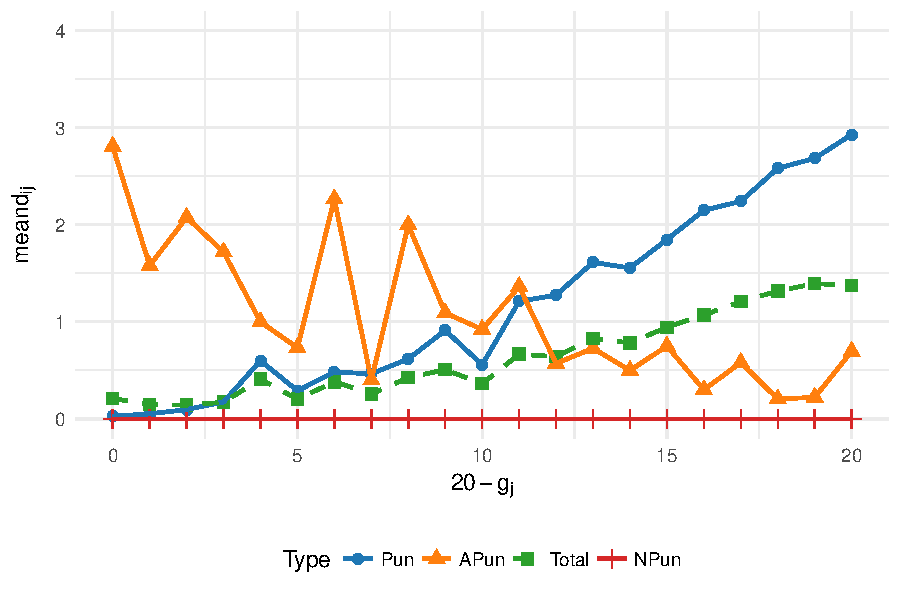
\includegraphics[width=.6\linewidth,clip,viewport={0 30 430 280}]{img/41_type}
  \raisebox{7.7em}{
  \begin{tabular}{c c r r}
         & Type  & N   & \%    \\ 
\midrule
 \lpun   & Pun   & 111 & 48.7  \\   
 \lnpun  & NPun  & 88  & 38.6  \\   
 \lapun  & APun  & 13  & 5.7   \\   
         & NCL   & 16  & 7.0   \\   
\midrule
 \ltotal & Total & 228 & 100.0 \\   
\bottomrule
  \end{tabular}
  }
  \label{fig:rpstype}
        \parbox{.95\textwidth}{\footnotesize \textit{Notes:} Punishment type
          distribution and average punishment patterns (in the $20 - g_j$-space)
          in the RPS-game
          for the different types: pro-social punishers (\emph{Pun}),
          non-punishers (\emph{NPun}), anti-social punishers (\emph{APun}), and
          non-classified punishment profiles (\textit{NCL}). To ease
          illustration, the pattern for the latter is not plotted.} 
\end{figure}

\subsection{Weakest Link Game Punishment Types}
%
In a next step we classify individual level sanctioning behavior in a weakest
link game setting. As documented by \cite{Lec2015} subjects engage in
costly peer-sanctions in coordination game environments as a means to foster
coordination. In line with their findings, we too observe considerable
sanctions in the weakest link game setting (WPS). Figure~\ref{fig:wpstype} shows
the distribution of types and their respective average sanctioning behavior in
the WPS-game. We observe an
increase in pro-socially sanctioning \emph{Pun}-types compared to the public
goods setting. 53.1\% of subjects sanction peers displaying low effort levels
more strongly than if they display larger efforts. We further observe a
reduction in non-sanctioning \emph{NPun} (30.3\%) and anti-socially sanctioning
\emph{APun} (3.1\%) individuals. Finally we observe an increase in
non-classifiable individuals (13.6\%).
%
% WPS punishment types
\begin{figure}[tbp]
  \caption{WPS-game Punishment Types}
  \centering
  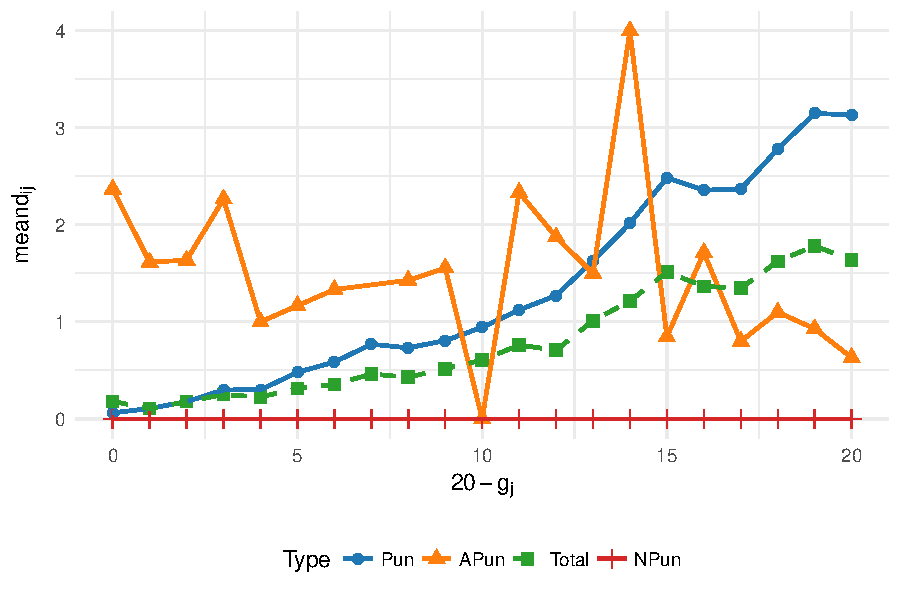
\includegraphics[width=.6\linewidth,clip,viewport={0 30 430 280}]{img/61_type}
  \raisebox{7.7em}{
  \begin{tabular}{c c r r}
         & Type  & N   & \%    \\ 
\midrule
 \lpun   & Pun   & 121 & 53.1  \\   
 \lnpun  & NPun  & 69  & 30.3  \\   
 \lapun  & APun  & 7   & 3.1   \\   
         & NCL   & 31  & 13.6  \\   
\midrule
 \ltotal & Total & 228 & 100.0 \\   
\bottomrule
  \end{tabular}
  }
  \label{fig:wpstype}
        \parbox{.95\textwidth}{\footnotesize \textit{Notes:} Punishment type
          distribution and average punishment patterns (in the $20 - g_j$-space)
          in the RPS-game
          for the different types: pro-social punishers (\emph{Pun}),
          non-punishers (\emph{NPun}), anti-social punishers (\emph{APun}), and
          non-classified punishment profiles (\textit{NCL}). To ease
          illustration, the pattern for the latter is not plotted.} 
\end{figure}


\subsection{Individual Cross-Domain Punishment Behavior}
%
Combining the two punishment classifications across the two
domains allows us to elicit the \emph{individual punishment type stability}.
Figure~\ref{fig:punXtab} shows the results. The majority (67.7\%) of subjects show a
consistent punishment type across the two domains. This includes Pun, NPun, and
APun types. Among the switchers the majority of subjects appears to be changing
their punishment behavior to be more pro-social. 21 subjects that exert no
punishment in the RP-game display a pro-social pattern in the WPS-game. 
% 2D RPS WPS Types
\begin{figure}[tbp]
  \centering
  \caption{Type Dristribution RPS- and WPS-game}
  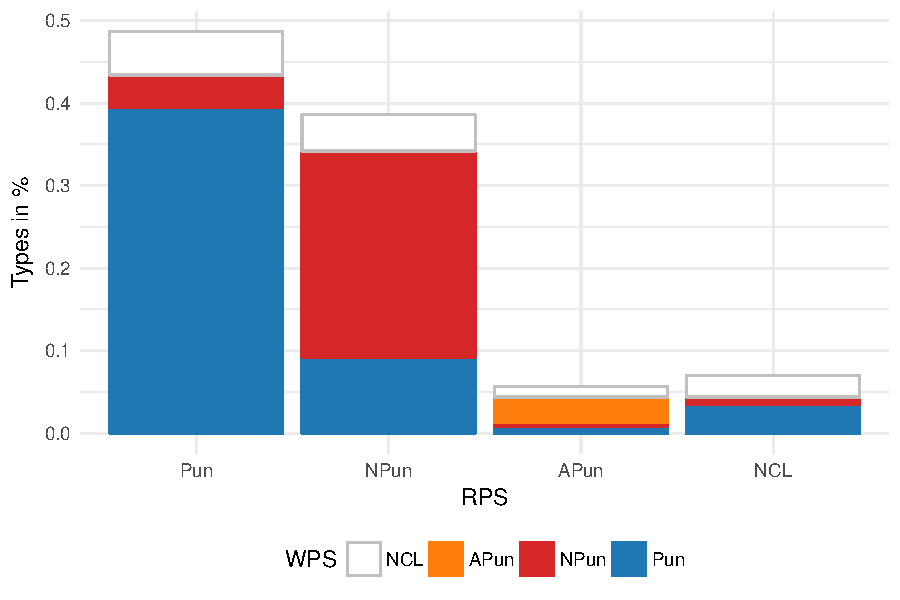
\includegraphics[width=.49\linewidth]{img/2d_types}
  \raisebox{8em}{
    \resizebox{.49\linewidth}{!}{
  \begin{tabular}[h]{r|cccc|c}
   \mco{1}{}       & \mco{4}{\emph{WPS-game}} &                                                                           \\
\emph{RPS} $\downarrow$ & Pun                     & NPun            & APun                    & NCL            & Total        \\
\midrule
Pun       & \nc 90                  & 9               & \color{gray} 0          & 12             & 111          \\
\fns\%    & \nc \fns [39.5]         & \fns [3.9]      & \fns \color{gray} [0.0] & \fns [5.3]     & \fns [48.7]  \\
NPun      & 21                      & \nc 57          & \color{gray} 0          & 10             & 88           \\
\fns\%    & \fns [9.2]              & \nc \fns [25.0] & \fns \color{gray} [0.0] & \fns [4.4]     & \fns [38.6]  \\
APun      & 2                       & 1               & \nc 7                   & 3              & 13           \\
\fns\%    & \fns [0.9]              & \fns [0.4]      & \nc \fns [3.1]          & \fns [1.3]     & \fns [5.7]   \\
NCL       & 8                       & 2               & \color{gray} 0          & 6          & 16           \\
\fns\%    & \fns [3.5]              & \fns [0.9]      & \fns \color{gray} [0.0] & \fns [2.6] & \fns [7.0]   \\
\midrule
Total     & 121                     & 69              & 7                       & 31             & 228          \\
\fns\%    & \fns [53.1]             & \fns [30.3]     & \fns [3.1]              & \fns [13.6]    & \fns [100.0] \\
 \bottomrule 
  \end{tabular}
  }
}
  \label{fig:punXtab}
  \smallskip                                                                                                    \\
  \parbox{\linewidth}{\footnotesize\textit{Note:} More than 65\% of subjects
    remain consistent across these two games in their punishment behavior.}
\end{figure}

\section{Joint Punishment Demand}

It remains to be seen whether this individual behavioral change translates into
differences in global punishment demand in the two settings (RPS and WPS).
Table~\ref{tab:avgPun} presents the results for pseudo panel regressions with
individual level fixed effects for the
two strategy method settings. Game and screen order are used as time variance to
construct the pseudo panel and capture potential ordering effects. As
figure~\ref{fig:rpstype} and figure~\ref{fig:wpstype} indicated we find significant positive
punishment demands for deviations from fully contributing one's endowment
(highest potential effort level) for both settings (RPS and WPS) in the respective estimations in column 1 and
2. The demand for sanctions in the WPS game appears hereby to be larger than the
demand for punishment in the RPS game. The estimation in column 3 supports this.
The interaction effect $D.WPS\times (20-g_j)$ in column 3 is positive and
significant on the 5 percent level indicating harsher sanctions for every token
kept in the private account in the WPS game over the RPS game. 
%
% avgPun RPS vs WPS 
\begin{table}[tbp]
  \centering
  \caption{Punishment Demand Across Games}
 \begin{tabular}{l*{4}{d{5}}}
\toprule
                       & \mco{4}{Assigned Punishment $d_{ij}$}                                 \\
                       & \mco{1}{RPS}    & \mco{1}{WPS}    & \mco{1}{Joint}  & \mco{1}{Stable} \\
                       & \mco{1}{(1)}    & \mco{1}{(2)}    & \mco{1}{(3)}    & \mco{1}{(4)}    \\
\midrule
$(20-g_j)$             & 0.068^{***}     & 0.085^{***}     & 0.068^{***}     & 0.086^{***}     \\
                       & (0.007)         & (0.007)         & (0.007)         & (0.009)         \\
[.3em]
$D.WPS$                &                 &                 & -0.017          & 0.030           \\
                       &                 &                 & (0.031)         & (0.029)         \\
[.3em]
$D.WPS\times (20-g_j)$ &                 &                 & 0.017^{**}      & 0.001           \\
                       &                 &                 & (0.007)         & (0.006)         \\
[.3em]
Intercept              & -0.005          & -0.019          & -0.000          & -0.055          \\
                       & (0.067)         & (0.070)         & (0.062)         & (0.083)         \\
\midrule
Observations           & \mco{1}{6,840}  & \mco{1}{6,840}  & \mco{1}{13,680} & \mco{1}{9,240}  \\
adj.\(R^{2}\)          & 0.222           & 0.251           & 0.201           & 0.263           \\
\textit{AIC}           & \mco{1}{18,036} & \mco{1}{19,974} & \mco{1}{41,357} & \mco{1}{26,656} \\
\textit{BIC}           & \mco{1}{18,043} & \mco{1}{19,980} & \mco{1}{41,379} & \mco{1}{26,677} \\
\bottomrule
\end{tabular}
  \label{tab:avgPun}
\end{table}

However, this does not reveal from where these additional sanctions stem. As
stated above despite remarkable punishment type stability within the
experimental subjects we still observe considerable behavioral fluctuations
between the two settings. We therefore investigate whether the additional
demand for sanctions is an expression of all subjects adapting their sanctioning
behavior to the new incentives or just a sub-population, and if this behavioral
adaptation is potentially already fully reflected in the two-domain punishment
classification.

Column 4 in table~\ref{ap:tab:avgPun} presents the results for a pooled RPS and
WPS estimation reduced to
the $154$ \emph{type-stable} subjects (Pun, NPun, APun) along the main diagonal
excluding NCL. The demand for
punishment $(20-g_j)$ increases slightly with respect to column 3 and can be
explained with the fact that the majority of stable individuals are Pun-type
subjects that generate the bulk of positive punishment demand. More
interestingly, none of the other coefficients remain significant on any conventional level.
This indicates that type-stable subjects are \emph{not} the driver of
the increased punishment demand in the WPS game, meaning that the increased
demand for sanctions are a result of individuals that change their sanctioning
behavior across the two domains.


\section{Contribution and Punishment Domain}

In the previous sections we studied the distribution of punishment types across
a linear public good game and a weakest link game. We will now continue to
cross-link these punishment classifications with individually elicited
contribution types.

\subsection{Contribution Types}
  
 In similar fashion to
\cite{Albrecht2016a} we use the C-game observations to classify contribution
types in the tradition of \cite{Fischbacher2001}.
We follow \cite{Albrecht2016a} in that we too classify subjects using linear
regression results, deviating from the original \cite{Fischbacher2001}, who use Spearman rank correlation.
In the C-game subjects had to decide upon their \emph{conditional contribution}
decision with respect to 21 displayed possible group mean contributions.
For each individual we estimate equation~\ref{eq:cctypes} in which the average
contribution of the other three group member $\overline{g}_{j}$ explains the
individual contribution decision $g_i$.
\begin{align}
  \label{eq:cctypes}
  g_i = a_i + b_i \overline{g}_{j} + e_i
\end{align}
Subjects are then classified in accordance with~\ref{Albrecht2016a}, i.e.,
\emph{Conditional Contributors} (CC) show a positive slope coefficient $b_i$,
significant on the 1 percent level, \emph{Free Rider} (FR) do not make positive
contributions in any of the 21 decision situations, \emph{Triangular
  Contributors} (TC) show a pattern that initially increases but starts to
decrease at a certain point.\footnote{As in~\ref{Fischbacher2001}
  and~\ref{Albrecht2016a} we classify TC types via eyeballing.} Similar to the the punishment classification an
additional group is introduced to capture behavioral patterns that do not fit
with any of the previous groups (NC).
Figure~\ref{fig:cctypes} presents the results for the contribution type classification.
A large majority of subjects (65.4\%) show upward sloping contribution patterns
and are classified as conditional contributors (CC). Another 18.4\% of individuals do
not transfer positive amounts to the public goods for any of the 21 group
contribution means (FR). Another 9.6\% of subjects are classified via eyeballing as triangular
contributors (TC). Finally 6.6\% individuals did no fit with any of the previous 3
classifications and were labeled an non-classifieds (NC). 

\FA{Usefull ?}
In a next step we combine these elicited contribution patterns with the previously
classified individual punishment patterns to two- and three-dimensional classifications.

% WPS punishment types
\begin{figure}[tbp]
  \caption{C-game Contribution Types}
  \centering
  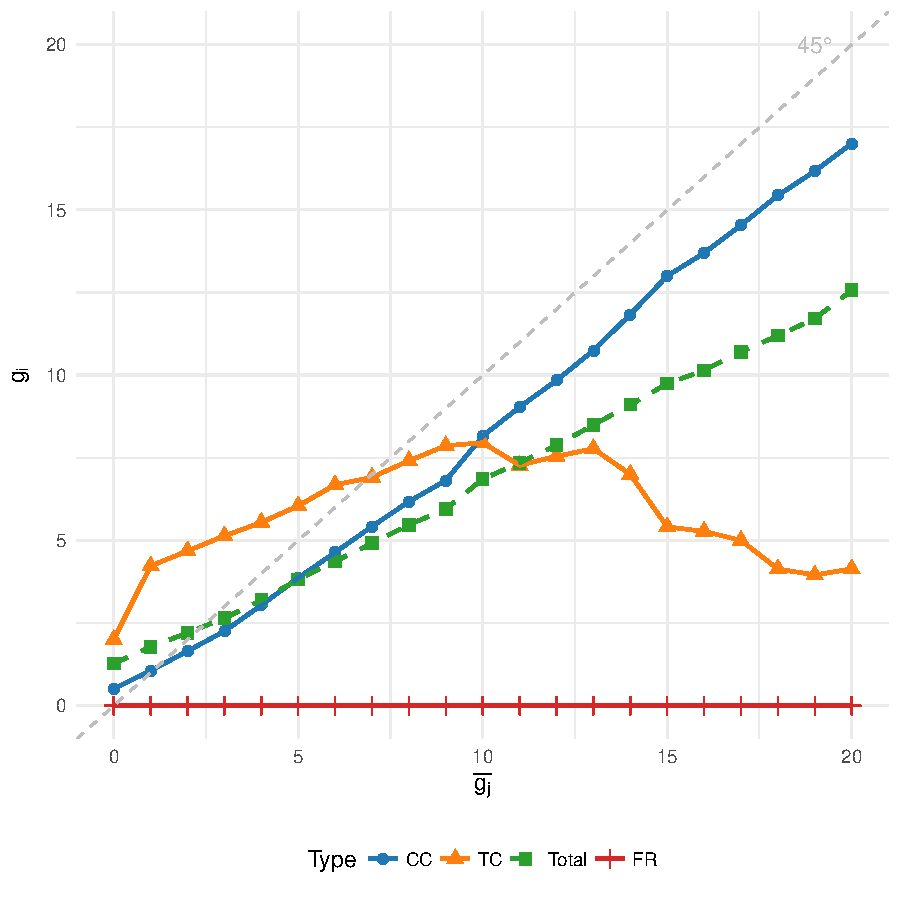
\includegraphics[width=.5\linewidth,clip,viewport={0 30 430 450}]{img/51_type}
  \raisebox{7.3em}{
  \begin{tabular}{c c r r}
         & Type  & N   & \%    \\ 
\midrule
 \lpun   & CC    & 149 & 65.4  \\   
 \lnpun  & FR    & 42  & 18.4  \\   
 \lapun  & TC    & 22  & 9.6   \\   
         & NC    & 15  & 6.6   \\   
\midrule
 \ltotal & Total & 228 & 100.0 \\   
\bottomrule
  \end{tabular}
  }
  \label{fig:cctypes}
    \parbox{.95\textwidth}{\footnotesize\textit{Notes:} The figure presents the distribution of contribution types, following \cite{Fischbacher2001} and \cite{Fischbacher2010}, and the average cooperation patterns for the different types: \textit{Conditional Cooperators (CC)}, \textit{Free-Riders (FR)}, \textit{Triangular Contributors (TC)}, and \textit{Non-classified (NC)} cooperation patterns. To ease illustration, the pattern for the latter is not plotted.}
\end{figure}

\subsection{Contribution $\times$ Punishment Types}

In the 

% CC vs PUN RPS
\begin{table}[htbp]
  \caption{Contribution $\times$ Punishment Type (C/RPS)}
  \centering
  \begin{tabular}{r|cccc|c}
  \mco{1}{}       & \mco{4}{C-Game} &                                                  \\ 
RPS  $\downarrow$ & CC              & FR         & TC        & NC        & Total       \\
\midrule
Pun               & 85              & 18         & 5         & 3         & 111         \\
\fns \%           & \fns[37.3]      & \fns[7.9]  & \fns[2.2] & \fns[1.3] & \fns[48.7]  \\
[.3em]          
  NPun            & 48              & 23         & 9         & 8         & 88          \\
\fns \%           & \fns[21.1]      & \fns[10.1] & \fns[4.0] & \fns[3.5] & \fns[38.6]  \\
[.3em]         
  APun            & 7               & 1          & 3         & 2         & 13          \\
\fns \%           & \fns[3.1]       & \fns[0.4]  & \fns[1.3] & \fns[0.9] & \fns[5.7]   \\
[.3em]        
NCL               & 9               & 0          & 5         & 2         & 16          \\
\fns \%           & \fns[4.0]       & \fns[0.00] & \fns[2.2] & \fns[0.9] & \fns[7.0]   \\
\midrule         
Total             & 149             & 42         & 22        & 15        & 228         \\
\fns \%           & \fns[65.4]      & \fns[18.4] & \fns[9.7] & \fns[6.6] & \fns[100.0] \\
\bottomrule
  \end{tabular}
  \label{tab:ccpunRPS}
\end{table}

% CC vs PUN WPS
\begin{table}[htbp]
  \caption{Contribution $\times$ Punishment Type (C/WPS)}
  \centering
  \begin{tabular}{r|cccc|c}
  \mco{1}{}       & \mco{4}{C-Game} &                                                  \\ 
WPS  $\downarrow$ & CC              & FR         & TC        & NC        & Total       \\
\midrule
Pun               & 89              & 22         & 7         & 3         & 121         \\
\fns \%           & \fns[39.0]      & \fns[9.7]  & \fns[3.1] & \fns[1.3] & \fns[53.1]  \\
[.3em]          
  NPun            & 42              & 13         & 9         & 5         & 69          \\
\fns \%           & \fns[18.4]      & \fns[5.7]  & \fns[4.0] & \fns[2.2] & \fns[30.3]  \\
[.3em]         
  APun            & 3               & 0          & 3         & 1         & 7           \\
\fns \%           & \fns[1.3]       & 0.0        & \fns[1.3] & 0.44      & \fns[3.1]   \\
[.3em]        
NCL               & 15              & 7          & 3         & 6         & 31          \\
\fns \%           & \fns[6.6]       & \fns[3.1]  & \fns[1.3] & \fns[2.6] & \fns[13.6]  \\
\midrule         
Total             & 149             & 42         & 22        & 15        & 228         \\
\fns \%           & \fns[65.4]      & \fns[18.4] & \fns[9.7] & \fns[6.6] & \fns[100.0] \\
\bottomrule
  \end{tabular}
  \label{tab:ccpunWPS}
\end{table}

\clearpage

\section{Impact of Type Prevalence on Group Outcomes}

To recap we found that individuals are heterogeneous in their punishment
behavior in two different game settings. The majority of subjects, when classified with a fairly simple approach,
remain type-stable across the two settings despite differing incentive
structures. We further find that the average demand for sanctions within the
weakest link setting (WPS) is significantly larger than in the linear public goods
setting (RPS) and that this increased demand stems from type-switching
individuals, who on average increase their demand for sanctions, while the
type-stable individual show no change in sanctioning demand.

We will now investigate the impact of the elicited behavioral types (punishment
and cooperation) on group success. In the case of
the 10 period repeated linear public good RP-game group success is measured in
increased average contributions and
increased average payoffs. For the 10 period repeated weakest link WP-game we
are concerned with improved efficiency, i.e., improved coordination on
\emph{any} or on the \emph{payoff-dominant} equilibrium.
%Additionally we use the
%reduction in unrefunded tokens\footnote{In the weakest link game tokens
%  transferred to the public good that are above the group's minimum transfer are
%not refunded and are lost to a group's welfare.} to investigate non-equilibrium
%efficiency gains. This is interesting as tacit equilibrium coordination is a
%daunting task \ldots.

We use the group composition of Pun and CC-type
individuals, as classified in the RPS, WPS
and C-game, resulting from the randomized assignment to experimental groups at the beginning of
the RP and WP-game as exogenous variation to test their respective impact on
group success.\footnote{Section~\ref{ap:sec:monte} in the
  supporting online materials shows the hypothetical distribution of Pun and
  CC-type subjects by running Monte Carlo simulations with 10,000 random draws
  from the observed individual type distribution in the C, RPS, and WPS-game
  with randomized assignment into groups of 4. The created hypothetical
  distributions is tested against our observed distributions using $\chi^2$-tests. We find no
  significant differences between the hypothetical and observed distributions (\textbf{Numbers}).}

\subsection{Cooperation Outcomes (RP-game)}
    % contribution punishment payoff
\begin{figure}[tbp]
  \centering
  \begin{tabular}{|c |c | c|}
    \hline
    Mean Contribution $\bar{g}_i$ (A)&
        Mean Punishment $\bar{d}_{ij}$ (B)& 
            Mean Payoff $\bar{\pi}_i$ (C)\\
    [.3em]
    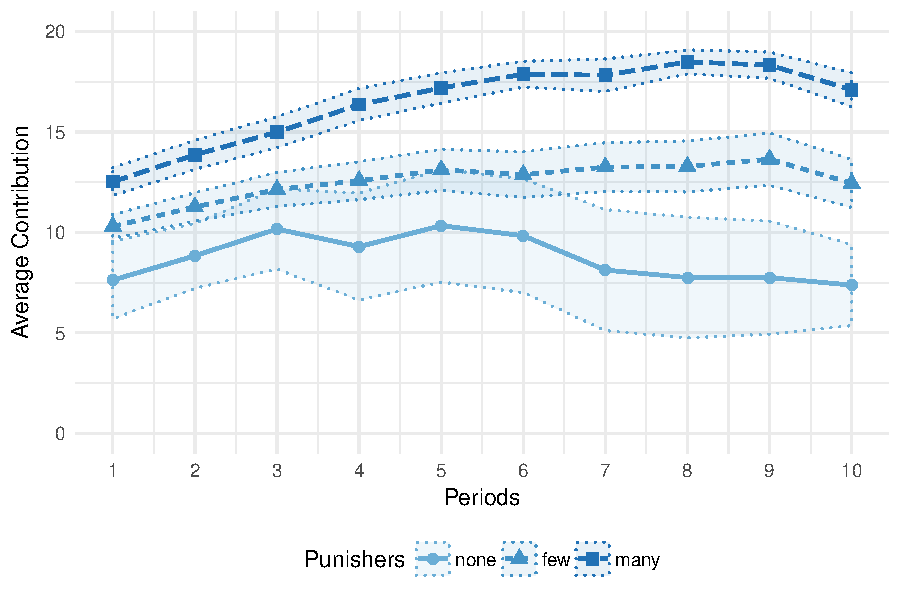
\includegraphics[width=.32\linewidth]{img/21_contrib} &
        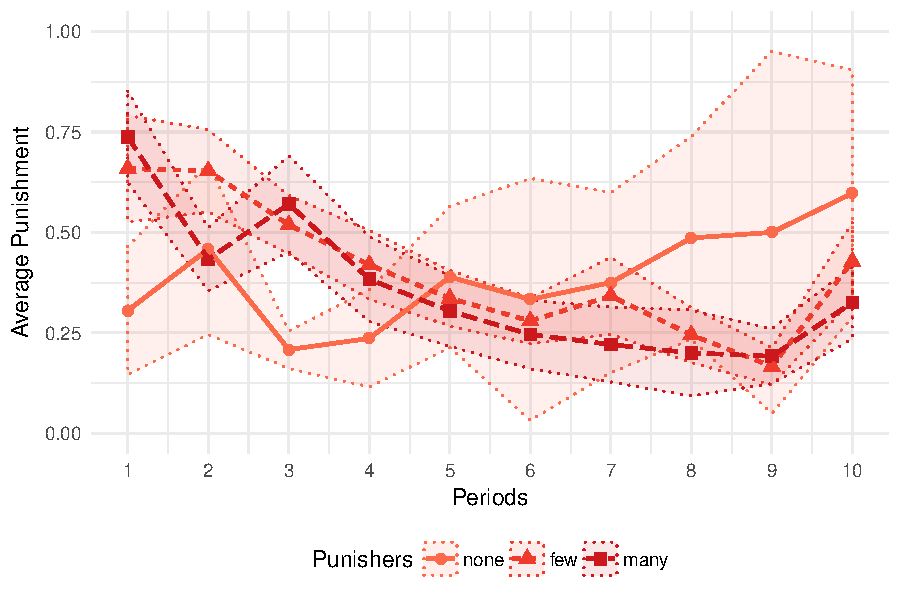
\includegraphics[width=.32\linewidth]{img/21_pun} &
            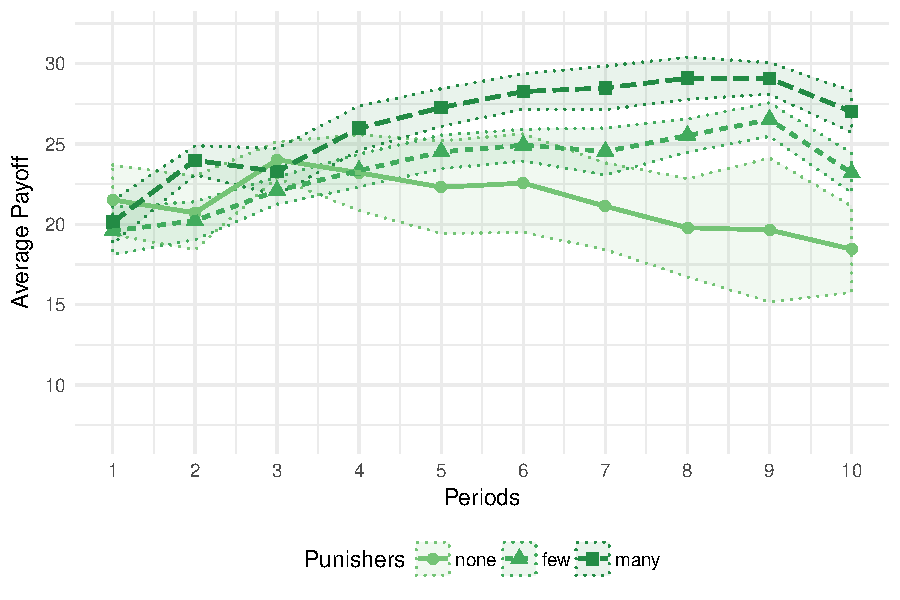
\includegraphics[width=.32\linewidth]{img/21_payoff}\\
    \hline
  \end{tabular}
  \caption{Average Group Outcomes by Type Prevalence in RP-game}
  \label{fig:groupoutRP}
  \smallskip
  \parbox{\linewidth}{\footnotesize\textit{Note:} Panel A shows the development
    of mean contributions to the public good over the 10 periods of the linear
    public good RP-game by Pun-type prevalence per group. Panel B depicts the
    mean punishment assigned to other group members, panel C the mean individual
  payoff subjects received. The 20 groups containing 3 or 4 Pun-type subjects
  are jointly depicted as \emph{many}, the 31 groups with 1 or 2 Pun-types as
  \emph{few}. The 6 groups without Pun-types are depicted separately.
  Figure~\ref{ap:fig:groupoutRP} in the supporting online material plots
  group compositions separately.}
\end{figure}

% cooperation in RP
\begin{table}[htbp]
  \caption{Cooperation in the RP-game}
  \centering
  \resizebox{\linewidth}{!}{
\begin{tabular}{r*{3}{d{5}}p{1em}*{3}{d{5}}}
\toprule
             & \mco{3}{Mean Contribution $\bar{g}_i$} &                & \mco{3}{Mean Payoff $\bar{\pi}_i$}                                              \\
             & \mco{1}{(1)}                  & \mco{1}{(2)}   & \mco{1}{(3)}   &  & \mco{1}{(4)}   & \mco{1}{(5)}   & \mco{1}{(9)}   \\
  \midrule
No.~of Pun   & 2.228^{***}                   &                & 1.997^{***}    &  & 1.350^{**}     &                & 1.349^{**}     \\
             & (0.537)                       &                & (0.573)        &  & (0.567)        &                & (0.577)        \\
[.3em]
No.~of CC    &                               & 1.644^{**}     & 0.817          &  &                & 0.560          & 0.002          \\
             &                               & (0.677)        & (0.746)        &  &                & (0.616)        & (0.673)        \\
[.3em]
Constant     & 9.144^{***}                   & 9.185^{***}    & 7.457^{***}    &  & 21.584^{***}   & 22.747^{***}   & 21.580^{***}   \\
             & (1.450)                       & (1.966)        & (2.150)        &  & (1.337)        & (1.584)        & (1.847)        \\
  \midrule
Obs.         & \mco{1}{570}                  & \mco{1}{570}   & \mco{1}{570}   &  & \mco{1}{570}   & \mco{1}{570}   & \mco{1}{570}   \\
\(R^{2}\)    & 0.222                         & 0.082          & 0.239          &  & 0.091          & 0.011          & 0.091          \\
\textit{AIC} & \mco{1}{2,949}                & \mco{1}{2,958} & \mco{1}{2,950} &  & \mco{1}{3,538} & \mco{1}{3,543} & \mco{1}{3,540} \\
\textit{BIC} & \mco{1}{2,966}                & \mco{1}{2,976} & \mco{1}{2,971} &  & \mco{1}{3,556} & \mco{1}{3,560} & \mco{1}{3,562} \\

\bottomrule
\end{tabular}
}
  \label{tab:coopRP}
  \smallskip\\
  \parbox{\linewidth}{\footnotesize\textit{Note:} Random effects panel estimation
    for 57 groups of 4 subjects over 10 periods. The explanatory
    variables can take values from 0 to 4. Columns 1-3 show estimation results
    for the impact of type prevalence on average contributions.
    Columns 4-6 show results for the impact on average payoffs. P-values: 0.1 /
    0.05 / 0.01 : * / ** / ***. Cluster robust standard errors in parentheses.
    }
\end{table}

In this chapter we replicate the results of \cite{Albrecht2016a}.
To elicit the impact of Pun-types on group cooperation we use the individual punishment
classification resulting from the RPS-game and the contribution classification
from the C-game.
Figure~\ref{fig:groupoutRP} shows the development over the ten periods in terms
of mean contribution $\bar{g}_i$ (A), mean assigned punishment $\bar{d}_{ij}$
(B), and mean payoff $\bar{\pi}_i$ (C) given the prevalence of pro-social
punishers in the respective groups. We reduced the five possible group
compositions into straight-forward cluster groups to ease
viewing.\footnote{Figure~\ref{ap:fig:groupoutRP} in the supporting online
  material shows graphs for all group compositions separately.} The 6 groups
\emph{without} Pun-type subjects remained separately as `none'. We joined groups
with one (14 groups)
or two (17 groups) Pun-types into the category `few' as these contained less than 50\%
Pun-types. Further we gathered groups with three (17 groups) or four (3 groups)
Pun-types in the category `many' as they contain more than 50\% of Pun-types.

In panel A of figure~\ref{fig:groupoutRP}  it is apparent that groups with
\emph{many} Pun-type subjects increase their contributions over the course of
the 10 periods of the RP-game and also the resulting payoffs appear to be
highest in the second half of the RP-game for groups with many pro-social
punishers.

Table~\ref{tab:coopRP} presents panel estimation results that support these
visual findings. Columns 1-3 show estimates for the impact on mean 
contributions $\bar{g}_i$ and columns 4-6 for mean payoffs $\bar{\pi}_i$.
Increasing numbers of pro-social punishers per group show a significant positive
effect on the level of mean contributions and on the level of mean payoffs.
Moreover the results suggest that the number of conditional contributors does
not enhance within group contribution levels. This is finding is further
supported by the low explanatory power (R$^\text{2}$) of models 2 and 5 and the increases
in the Akaike and Bayesian information criterion in models 2 and 3 (5 and 6)
compared to model 1 (4). Our findings are similar with the
difference that \emph{many} CC-types show a significant impact in
\cite{Albrecht2016a}.\footnote{Contrary to \ref{Albrecht2016a} we used the
  number of Pun and CC-type subjects in their linear form to perform our
  estimations. This was necessary as the distribution of group compositions in
  the margins -- 6 groups without Pun-types, 1 group without CC-types -- did not
  warrant separation by clusters using dummy variables. Nevertheless, the
  graphical representations support the general findings of the regression models.} 


\subsection{Coordination}
    % equilibria distribution

Turning to the weakest link game we now want to investigate group success in a
coordination setting. Contrary to the public goods game where zero contribution
is the sole subgame perfect Nash-equilibrium, in the weakest link game every
joint equal effort level (contribution level) for the public good is a
Nash-equilibrium. These equilibria are pareto ranked from contributing nothing being
the least efficient to contributing fully being the payoff-dominant
Nash-equilibrium.


    % contribution punishment payoff
\begin{figure}[tbp]
  \centering
  \begin{tabular}{|c|c|c|}
    \hline
    Minimum Contribution $min({g})_i$ &
        Average Punishment $\bar{d}_{ij}$ & 
            Average Payoff $\bar{\pi}_i$\\
    [.3em]
    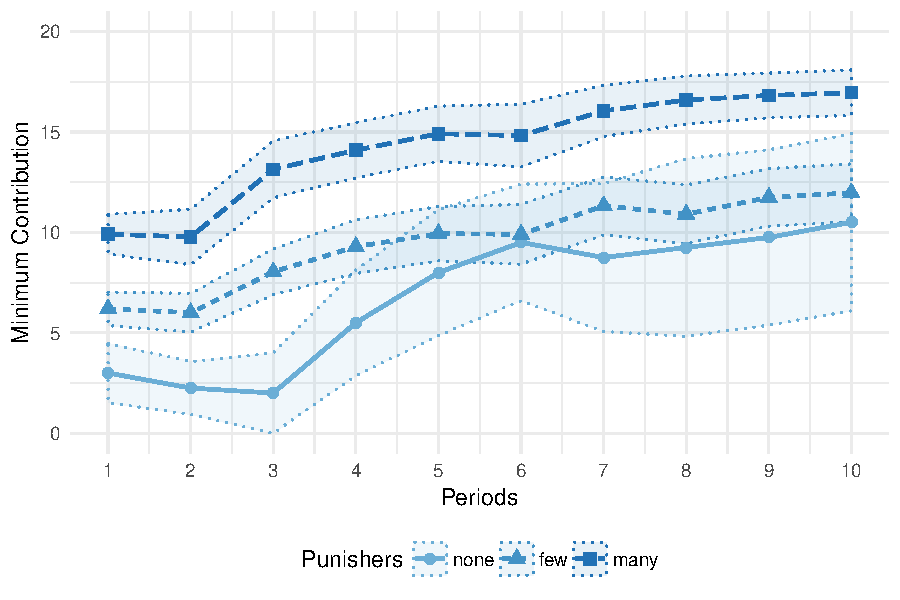
\includegraphics[width=.3\linewidth]{img/71_minimum} &
        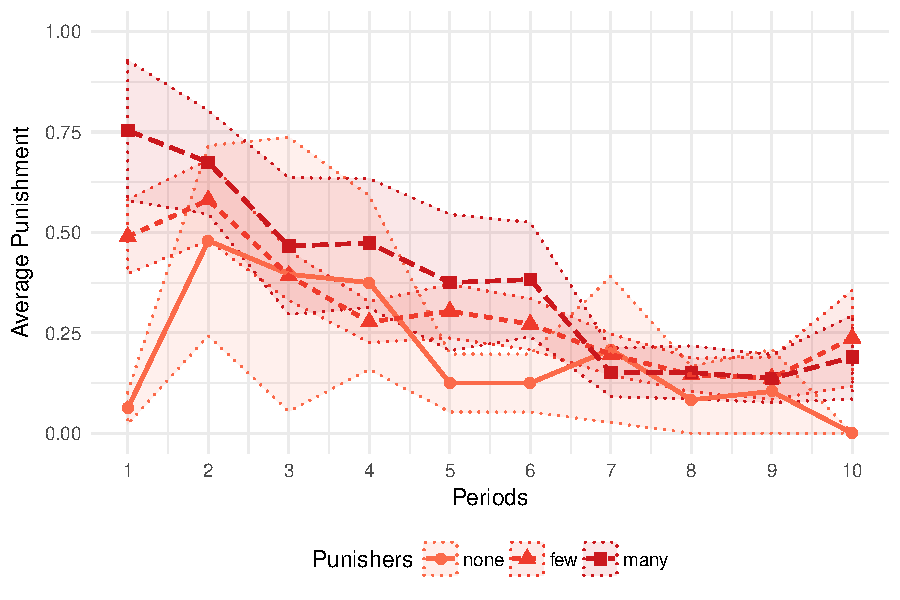
\includegraphics[width=.3\linewidth]{img/71_pun} &
            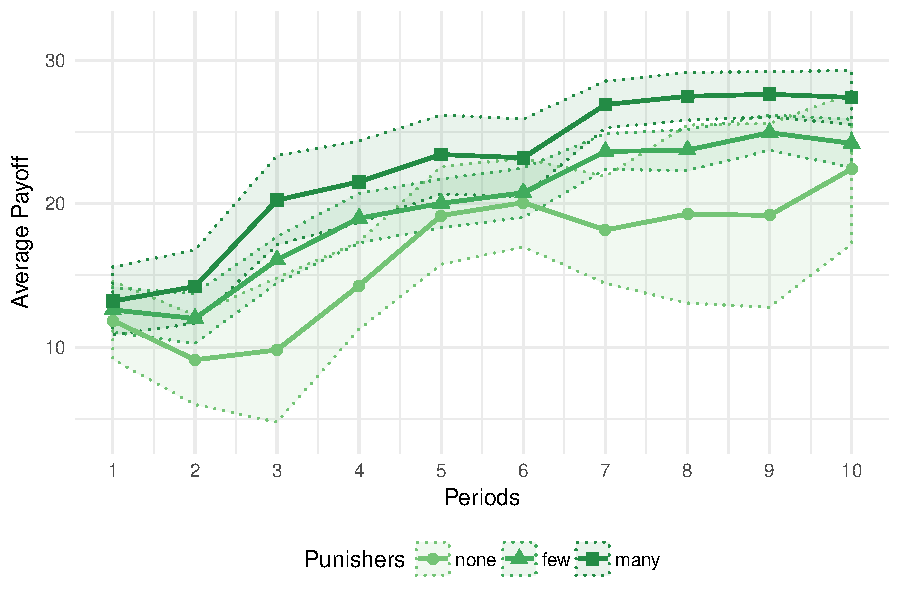
\includegraphics[width=.3\linewidth]{img/71_payoff}\\
    \hline
  \end{tabular}
  \caption{Average Group Outcomes by Type Prevalence in WP-game}
  \label{fig:groupoutWP}
  \smallskip
  \parbox{\linewidth}{\footnotesize\textit{Note:} Panel A shows the development
    of minimum contributions to the public good over the 10 periods of the linear
    public good RP-game by Pun-type prevalence per group. Panel B depicts the
    mean punishment assigned to other group members, panel C the mean individual
  payoff subjects received. The 20 groups containing 3 or 4 Pun-type subjects
  are jointly depicted as \emph{many}, the 31 groups with 1 or 2 Pun-types as
  \emph{few}. The 6 groups without Pun-types are depicted separately.
  Figure~\ref{ap:fig:groupoutWP} in the supporting online material plots
  group compositions separately.}
\end{figure}
 
    % equilibrium distribution
\begin{figure}[tbp]
  \centering
  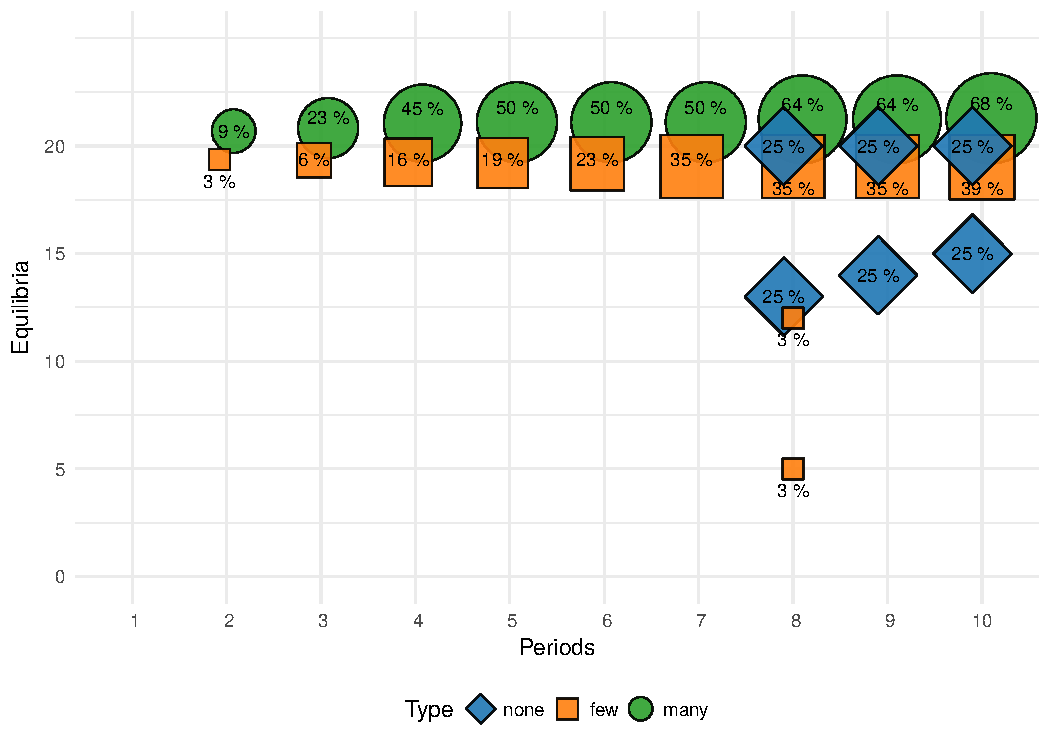
\includegraphics[width=0.49\linewidth]{img/equi_bubble} 
  \caption[Distribution of Equilibria]{Distribution of Equilibrium Coordination by Type Prevalence}
  \label{fig:equibub}
  \smallskip
  \parbox{\linewidth}{\footnotesize\textit{Note:} Fraction of
    successful equilibrium coordination by the 4 groups \emph{without} Pun-types
    (none), 33
    with \emph{few}, and 20 groups with \emph{many} Pun-type subjects, as
    classified based on WPS behavior. One group \emph{without} Pun-type subjects
    coordinates on the payoff dominant equilibrium in period 8, 9, and 10. A
    second group without Pun-types manages to coordinate on the not
    payoff-dominant equilibria 13, 14, and 15 in periods 8, 9, and 10. Groups with \emph{few} Pun-types
    coordinate twice on equilibria that are not payoff-dominant in period 8. In the majority of cases groups with
    \emph{few} Pun-types coordinate on the payoff-dominant equilibrium when
    successfully coordinating. Groups with \emph{many} Pun-types exclusively
    coordinate successfully on the payoff dominant equilibrium. All groups fail
    to tacitly coordinate on an equilibrium in the first period.}

  % group ID 11 none = equi == 20
 % group ID 40 none = equi = 13 ,14, 15  
\end{figure} 

% equilibrium coordination
\begin{table}[tbp]
  \caption{Equiblibrium Coordination in the WP-game}
  \centering
  \resizebox{\linewidth}{!}{
\begin{tabular}{r*{3}{d{5}}p{1em}*{3}{d{5}}}
\toprule
             & \mco{3}{Any Potential Equiblibrium} &              & \mco{3}{Payoff-Dominant Equilibrium}                         \\
             & \mco{1}{(1)}                        & \mco{1}{(2)} & \mco{1}{(3)} &  & \mco{1}{(4)} & \mco{1}{(5)} & \mco{1}{(9)} \\
\midrule
No.~of Pun   & 0.285                               &              & 0.220        &  & 0.697^{***}  &              & 0.635^{**}   \\
             & (0.188)                             &              & (0.210)      &  & (0.255)      &              & (0.281)      \\
[.3em]
No.~of CC    &                                     & 0.278        & 0.164        &  &              & 0.487^{*}    & 0.164        \\
             &                                     & (0.216)      & (0.238)      &  &              & (0.292)      & (0.314)      \\
[.3em]
Intercept    & -1.443^{***}                        & -1.572^{***} & -1.734^{***} &  & -2.822^{***} & -2.624^{***} & -3.120^{***} \\
             & (0.452)                             & (0.609)      & (0.625)      &  & (0.652)      & (0.841)      & (0.880)      \\
%\hline
%lnsig2u     &                                     &              &              &  &              &              &              \\
%Constant    & 0.444                               & 0.475        & 0.437        &  & 0.942^{***}  & 1.052^{***}  & 0.934^{***}  \\
%            & (0.304)                             & (0.303)      & (0.305)      &  & (0.331)      & (0.331)      & (0.331)      \\
\midrule
Obs.         & \mco{1}{570}                        & \mco{1}{570} & \mco{1}{570} &  & \mco{1}{570} & \mco{1}{570} & \mco{1}{570} \\
\textit{AIC} & \mco{1}{564}                        & \mco{1}{565} & \mco{1}{566} &  & \mco{1}{470} & \mco{1}{475} & \mco{1}{472} \\
\textit{BIC} & \mco{1}{577}                        & \mco{1}{578} & \mco{1}{583} &  & \mco{1}{483} & \mco{1}{488} & \mco{1}{489} \\
\bottomrule
\end{tabular}
}
  \label{tab:equiWPS}
  \smallskip\\
  \parbox{\linewidth}{\footnotesize\textit{Note:} Random effects panel probit
    estimation for 57 groups of 4 subjects over 10 periods. The explanatory
    variables can take values from 0 to 4. Columns 1-3 show estimation results
    for group coordinating on \emph{any} possible equilibrium in the game.
    Columns 4-6 show results for coordination on the \emph{payoff-dominant}
    equilibrium. P-values: 0.1 / 0.05 / 0.01 : * / ** / ***. Standard errors in parentheses.
    }
\end{table}

\clearpage
\printbibliography
\end{refsection}


% ------------------------------ Online Appendix ---------------------------------------------
\newpage
\appendix
\pagenumbering{arabic}

\begin{spacing}{1.15}

\setcounter{footnote}{0}
\renewcommand{\thesection}{\Roman{section}}\setcounter{section}{0}
%\renewcommand{\thesubsection}{\Roman{section}.\arabic{subsection}}
\renewcommand{\thesubsection}{\Roman{section}.\arabic{subsection}}\setcounter{subsection}{0}

\renewcommand{\thetable}{S.\arabic{table}} \setcounter{table}{0}
\renewcommand{\theequation}{S.\arabic{equation}} \setcounter{equation}{0}
\renewcommand{\thefigure}{S.\arabic{figure}} \setcounter{figure}{0}


%\addcontentsline{toc}{section}{Supplementary Appendix}
\begin{center}
  \textbf{\Large{Supporting Online Material}}\\ \normalsize{(\textsl{For Online Publication Only})}\bigskip\\
  { \Large {\textbf {\thetitle}}} \bigskip\\
  { \large {\theauthor }}\medskip\\
  \today \bigskip \\
   {\footnotesize$\dag$ University of Marburg; $\ddag$ University of Bonn; $\sharp$ Max Planck Institute for Research on Collective Goods; \mbox{$^*$ Hertie School of Governance}}
\end{center}

\tableofcontents
\listoftables
\listoffigures

\end{spacing}
\begin{refsection}

\section{Contribution Triplets}\label{ap:sec:triple}
Below we list the contribution triples that were used within each combination of $g^L$, $g^M$ and $g^H$ (see Table~\ref{tab:triplet}).
Before the experiment, these 10 $\times$ 8 triples were randomly generated by sampling with replacement from the corresponding sets $g^L$, $g^M$, $g^H$.
Each player then faced a randomly selected triple within each combination 1 -- 10.
If the selected triple would by chance correspond to the real triple, the subject would not face this situation but instead another one of the pre-defined contribution triples for the corresponding combination.\bigskip\\
%
\resizebox{\linewidth}{!}{
\begin{tabular}{*{10}c}
  &&(1)&(2)&(3)&(4)&(5)&(6)&(7)&(8)\\
(1)&($g^L$, $g^L$, $g^L$):& (0,0,0)& (0,2,3)& (1,1,3)& (1,2,2)& (1,2,3)& (1,2,4)& (1,3,3)& (1,3,4) \\ 
(2)&($g^L$, $g^L$, $g^M$):& (0,1,5)& (0,2,8)& (0,2,14)& (1,2,10)& (1,2,12)& (1,3,14)& (2,2,6)& (2,3,12)\\ 
(3)&($g^L$, $g^L$, $g^H$):& (0,3,18)& (1,2,20)& (1,3,19)& (1,4,20)& (2,2,18)& (2,2,19)& (3,3,18)& (4,4,17)\\ 
(4)&($g^L$, $g^M$, $g^M$):& (0,9,11)& (0,5,12)& (0,13,14)& (1,10,15)& (2,6,8)& (2,9,11)& (2,10,15)& (3,13,14)\\ 
(5)&($g^L$, $g^M$, $g^H$):& (0,6,19)& (0,14,17)& (2,6,17)& (2,8,20)& (2,11,19)& (3,7,18)& (4,8,17)& (4,10,20)\\ 
(6)&($g^L$, $g^H$, $g^H$):& (0,18,19)& (1,19,19)& (2,18,19)& (2,18,20)& (2,19,19)& (3,18,20)& (3,19,19)& (4,19,20)\\ 
(7)&($g^M$, $g^M$, $g^M$):& (5,7,12)& (5,14,16)& (6,6,9)& (6,10,10)& (7,8,9)& (7,10,13)& (7,14,16)& (8,9,11)\\ 
(8)&($g^M$, $g^M$, $g^H$):& (5,5,17)& (5,8,18)& (6,11,20)& (8,15,17)& (9,12,18)& (9,15,18)& (11,15,19)& (12,15,19) \\ 
(9)&($g^M$, $g^H$, $g^H$):& (5,18,20)& (7,18,19)& (9,18,20)& (11,17,17)& (12,17,18)& (12,18,18)& (14,17,20)& (15,17,19)\\ 
(10)&($g^H$, $g^H$, $g^H$):& (17,17,19)& (17,18,19)& (17,18,20)& (17,19,19)& (17,19,20)& (18,18,19)& (18,18,20)& (20,20,20)\\
\end{tabular}
}
% 
%\FA{Austausch der folgenden Triples für Bonn 2016:  \\\textbf{(M,M,M):} (5,14,16)\ra(5,14,15); (7,14,16) \ra(7,14,15);\\ \textbf{(M,M,H):} (5,8,18)\ra(5,8,16)}


\section{Instructions}

Below you find the English set of instructions used at FSU. The German and Japanese set of instructions can be requested from the authors.
The first part describes a public good game without punishment in the tradition of \citep{Fischbacher2001}, which was played ahead of the core games with punishment. The second part describes the \emph{One-Shot} game, the third the \emph{Repeated Interaction} game respectively.

%%%%%\addcontentsline{toc}{subsection}{Instructions}

%\includepdf[pages=-]{img/Part0}
%\includepdf[pages=-]{img/Part1}
%\includepdf[pages=-]{img/Part2}
%\includepdf[pages=-]{img/Part3}


\section{Contribution vs. Payoff Discussion}\label{ap:sec:con1pay}

\begin{table}[htbp]
  \centering
  \caption[Estimation Approach Discussion]{Contribution versus Payoff as
    Explanatory Variables}
\begin{tabular}{r*{4}{d{5}}}
  \toprule
  & \mco{4}{\it Individually Assigned Punishment $d_{ij}$}\\
                                 & \mco{2}{RPS}      & \mco{2}{WPS}                                                   \\
                                 & \mco{1}{(1)}      & \mco{1}{(2)}      & \mco{1}{(3)}      & \mco{1}{(4)}        \\
  \midrule
$(20-g_j)$                       & 0.068^{***}       &                   & 0.085^{***}       &                     \\
                                 & (0.007)           &                   & (0.007)           &                     \\
[.3em]
$\pi_j$                          &                   & 0.062^{***}       &                   & 0.038^{***}         \\
                                 &                   & (0.006)           &                   & (0.003)             \\
[.3em]
Intercept                        & -0.005            & -0.962^{***}      & -0.019            & 0.182^{***}         \\
                                 & (0.067)           & (0.158)           & (0.070)           & (0.057)             \\
\midrule
Observations                     & \mco{1}{6,840}    & \mco{1}{6,840}    & \mco{1}{6,840}    & \mco{1}{6,840}      \\
Adjusted \(R^{2}\)               & 0.222             & 0.098             & 0.251             & 0.048               \\
\textit{AIC}                     & \mco{1}{18,036}   & \mco{1}{19,054}   & \mco{1}{19,974}   & \mco{1}{21,619}     \\
  \textit{BIC}                   & \mco{1}{18,043}   & \mco{1}{19,061}   & \mco{1}{19,980}   & \mco{1}{21,626}     \\
  \bottomrule
\end{tabular}
  \label{ap:tab:con1pay}
  \smallskip\\
  \parbox{\linewidth}{\footnotesize\textit{Note:} Pseudo panel estimation with
    individual level fixed effects for 228 subjects. Cluster robust standard errors in
    parentheses.  P-values: 0.1 / 0.05 / 0.01 : * / ** / ***. Column (1), (3),
    and (5) only RP-game,
    (2), (4), and (6) only WP-game observations with 30 observations per
    subjects in each game.}
 % $g_i$ is individually constant within each
 %   game. Taking the difference $g_j$ and $g_i$ \emph{normalizes}
 %   observations of the P-, RP-, and WP-game creating a single kink
 %   for all three games.}
\end{table}

% contrib diff vs pay diff
\begin{table}[htbp]
  \centering
  \caption[Contribution Difference vs. Payoff Difference]{Contribution
    Difference vs. Payoff Difference as Explanatory Variables}
\begin{tabular}{r d{5}p{2ex}d{5} l}
  \toprule
                                 \mco{5}{\it Individually Assigned Punishment $d_{ij}$}                \\
                                 & \mco{1}{(1)}    &  & \mco{1}{(2)}    &                              \\
  \midrule
$max(\pi_j-\pi_i,0)$             & -0.008          &  & -0.008          & $max(g_j-g_i,0)$             \\
                                 & (0.006)         &  & (0.006)         &                              \\
[.3em]                                                                                      
$max(\pi_i-\pi_j,0)$             & 0.120^{***}     &  & 0.120^{***}     & $max(g_i-g_j,0)$             \\
                                 & (0.012)         &  & (0.012)         &                              \\
[.3em]                                                                                      
$D.WPS\times max(\pi_j-\pi_i,0)$ & -0.003          &  & -0.003          & $D.WPS\times max(g_j-g_i,0)$ \\
                                 & (0.006)         &  & (0.006)         &                              \\
[.3em]                                                                                      
$D.WPS\times max(\pi_i-\pi_j,0)$ & -0.004          &  & -0.004          & $D.WPS\times max(g_i-g_j,0)$ \\
                                 & (0.012)         &  & (0.012)         &                              \\
[.3em]
$D.min(g_{jkl})$                 & 0.278^{***}     &  & 0.278^{***}     & $D.min(g_{jkl})$             \\
                                 & (0.057)         &  & (0.057)         &                              \\
[.3em]
$D.WPS\times D.min(g_{jkl})$     & 0.043           &  & 0.043           & $D.WPS\times D.min(g_{jkl})$ \\
                                 & (0.072)         &  & (0.072)         &                              \\
[.3em]
Intercept                        & 0.061           &  & 0.061           & Intercept                    \\
                                 & (0.056)         &  & (0.056)         &                              \\
\midrule
Observations                     & \mco{1}{13,680} &  & \mco{1}{13,680} & Observations                 \\
Adjusted \(R^{2}\)               & 0.319           &  & 0.319           & Adjusted \(R^{2}\)           \\
\textit{AIC}                     & \mco{1}{39,175} &  & \mco{1}{39,175} & \textit{AIC}                 \\
  \textit{BIC}                   & \mco{1}{39,220} &  & \mco{1}{39,220} & \textit{BIC}                 \\
  \bottomrule
\end{tabular}
  \label{ap:tab:sdiffpay}
  \smallskip                                                                                           \\
  \parbox{\linewidth}{\footnotesize\textit{Note:} Pseudo panel estimation with
    individual level fixed effects for 228 subjects. Cluster robust standard errors in
    parentheses.  P-values: 0.1 / 0.05 / 0.01 : * / ** / ***. Column (1), (3),
    and (5) only RP-game,
    (2), (4), and (6) only WP-game observations with 30 observations per
    subjects in each game.}
 % $g_i$ is individually constant within each
 %   game. Taking the difference $g_j$ and $g_i$ \emph{normalizes}
 %   observations of the P-, RP-, and WP-game creating a single kink
 %   for all three games.}
\end{table}

\clearpage
\section{Additional Analyses}

\subsection{Self-Centered Punishment Classification}
% sdiff classification
\begin{table}[htbp]
  \centering
  \caption{Type Dristribution RP- and WP-game}
  \begin{tabular}[h]{rccccccccc}
\toprule
               & \mco{9}{t\_sdiff\_61}                                                                                                                                                                                     \\
t\_sdiff\_bz41 & -12                   & -10                   & -1                    & 0                     & 2                     & 20                    & 23                    & 100                   & Total     \\
\midrule
-11 No.        & \color{gray} 0        & 1                     & \color{gray} 0        & \color{gray} 0        & \color{gray} 0        & \color{gray} 0        & \color{gray} 0        & \color{gray} 0        & 1         \\
\%             & \fns \color{gray} 0.0 & \fns 0.4              & \fns \color{gray} 0.0 & \fns \color{gray} 0.0 & \fns \color{gray} 0.0 & \fns \color{gray} 0.0 & \fns \color{gray} 0.0 & \fns \color{gray} 0.0 & \fns 0.4  \\
-10 No.        & \color{gray} 0        & 50                    & \color{gray} 0        & 6                     & \color{gray} 0        & \color{gray} 0        & \color{gray} 0        & 6                     & 62        \\
\%             & \fns \color{gray} 0.0 & \fns 21.9             & \fns \color{gray} 0.0 & \fns 2.6              & \fns \color{gray} 0.0 & \fns \color{gray} 0.0 & \fns \color{gray} 0.0 & \fns 2.6              & \fns 27.2 \\
-1 No.         & \color{gray} 0        & \color{gray} 0        & 38                    & 3                     & \color{gray} 0        & \color{gray} 0        & \color{gray} 0        & 5                     & 46        \\
\%             & \fns \color{gray} 0.0 & \fns \color{gray} 0.0 & \fns 16.7             & \fns 1.3              & \fns \color{gray} 0.0 & \fns \color{gray} 0.0 & \fns \color{gray} 0.0 & \fns 2.2              & \fns 20.2 \\
0 No.          & \color{gray} 0        & 8                     & 14                    & 57                    & \color{gray} 0        & \color{gray} 0        & \color{gray} 0        & 9                     & 88        \\
\%             & \fns \color{gray} 0.0 & \fns 3.5              & \fns 6.1              & \fns 25.0             & \fns \color{gray} 0.0 & \fns \color{gray} 0.0 & \fns \color{gray} 0.0 & \fns 3.9              & \fns 38.6 \\
2 No.          & \color{gray} 0        & \color{gray} 0        & \color{gray} 0        & 1                     & 1                     & \color{gray} 0        & \color{gray} 0        & 1                     & 3         \\
\%             & \fns \color{gray} 0.0 & \fns \color{gray} 0.0 & \fns \color{gray} 0.0 & \fns 0.4              & \fns 0.4              & \fns \color{gray} 0.0 & \fns \color{gray} 0.0 & \fns 0.4              & \fns 1.3  \\
20 No.         & 1                     & \color{gray} 0        & \color{gray} 0        & \color{gray} 0        & \color{gray} 0        & 2                     & \color{gray} 0        & 3                     & 6         \\
\%             & \fns 0.4              & \fns \color{gray} 0.0 & \fns \color{gray} 0.0 & \fns \color{gray} 0.0 & \fns \color{gray} 0.0 & \fns 0.9              & \fns \color{gray} 0.0 & \fns 1.3              & \fns 2.6  \\
100 No.        & \color{gray} 0        & 7                     & 2                     & 2                     & \color{gray} 0        & \color{gray} 0        & 1                     & 10                    & 22        \\
\%             & \fns \color{gray} 0.0 & \fns 3.1              & \fns 0.9              & \fns 0.9              & \fns \color{gray} 0.0 & \fns \color{gray} 0.0 & \fns 0.4              & \fns 4.4              & \fns 9.6  \\
    \midrule
Total No.      & 1                     & 66                    & 54                    & 69                    & 1                     & 2                     & 1                     & 34                    & 228       \\
\%             & 0.4                   & 28.9                  & 23.7                  & 30.3                  & 0.4                   & 0.9                   & 0.4                   & 14.9                  & 100.0     \\
 \bottomrule 
  \end{tabular}
  \label{ap:tab:sdifftype}
  \smallskip  \\
  \parbox{\linewidth}{\footnotesize\textit{Note:}  }
\end{table}

% avgPun RPS vs WPS 
\begin{sidewaystable}
  \centering
  \caption{Punishment Demand}
 \begin{tabular}{l*{8}{d{5}}}
\toprule
                             & \mco{8}{Assigned Punishment $d_{ij}$}                                                                                                         \\
                             & \mco{1}{RPS}    & \mco{1}{WPS}    & \mco{1}{Joint}  & \mco{1}{stable} & \mco{1}{RPS}    & \mco{1}{WPS}    & \mco{1}{Joint}  & \mco{1}{stable} \\
                             & \mco{1}{(1)}    & \mco{1}{(2)}    & \mco{1}{(3)}    & \mco{1}{(4)}    & \mco{1}{(5)}    & \mco{1}{(6)}    & \mco{1}{(7)}    & \mco{1}{(8)}    \\
\midrule
$(20-g_j)$                   & 0.068^{***}     & 0.085^{***}     & 0.068^{***}     & 0.086^{***}     & 0.056^{***}     & 0.072^{***}     & 0.052^{***}     & 0.073^{***}     \\
                             & (0.007)         & (0.007)         & (0.007)         & (0.009)         & (0.007)         & (0.007)         & (0.007)         & (0.009)         \\
[.3em]
$D.WPS$                      &                 &                 & -0.017          & 0.030           &                 &                 & -0.025          & 0.026           \\
                             &                 &                 & (0.031)         & (0.029)         &                 &                 & (0.031)         & (0.030)         \\
[.3em]
$D.WPS\times (20-g_j)$       &                 &                 & 0.017^{**}      & 0.001           &                 &                 & 0.019^{***}     & 0.001           \\
                             &                 &                 & (0.007)         & (0.006)         &                 &                 & (0.007)         & (0.006)         \\
[.3em]
$D.min(g_{jkl})$             &                 &                 &                 &                 & 0.473^{***}     & 0.424^{***}     & 0.580^{***}     & 0.450^{***}     \\
                             &                 &                 &                 &                 & (0.051)         & (0.045)         & (0.064)         & (0.066)         \\
[.3em]
$D.WPS\times D.min(g_{jkl})$ &                 &                 &                 &                 &                 &                 & -0.130^{*}      & -0.030          \\
                             &                 &                 &                 &                 &                 &                 & (0.076)         & (0.078)         \\
[.3em]
Intercept                    & -0.005          & -0.019          & -0.000          & -0.055          & 0.025           & 0.009           & 0.036           & -0.027          \\
                             & (0.067)         & (0.070)         & (0.062)         & (0.083)         & (0.065)         & (0.069)         & (0.061)         & (0.082)         \\
\midrule
Observations                 & \mco{1}{6,840}  & \mco{1}{6,840}  & \mco{1}{1,3680} & \mco{1}{9,240}  & \mco{1}{6,840}  & \mco{1}{6,840}  & \mco{1}{1,3680} & \mco{1}{9,240}  \\
adj.\(R^{2}\)                & 0.222           & 0.251           & 0.201           & 0.263           & 0.246           & 0.267           & 0.223           & 0.280           \\
\textit{AIC}                 & \mco{1}{18,036} & \mco{1}{19,974} & \mco{1}{41,357} & \mco{1}{26,656} & \mco{1}{17,821} & \mco{1}{19,827} & \mco{1}{40,978} & \mco{1}{26,442} \\
\textit{BIC}                 & \mco{1}{18,043} & \mco{1}{19,980} & \mco{1}{41,379} & \mco{1}{26,677} & \mco{1}{17,835} & \mco{1}{19,841} & \mco{1}{41,016} & \mco{1}{26,477} \\
\bottomrule
\end{tabular}
  \label{ap:tab:avgPun}
\end{sidewaystable}

    % contribution punishment payoff
\begin{figure}[p]
  \centering
  \begin{tabular}{|c p{2ex} c|}
    \hline
    %\multicolumn{3}{|c|}{Average  } \\
    \multicolumn{3}{|c|}{\hspace{6ex}-- Average $\bar{g}_i$ --\hspace{10ex} Contribution \hspace{8ex}-- Minimum $min(g_i)$ --} \\
    A&&D\\
    [.5em]
    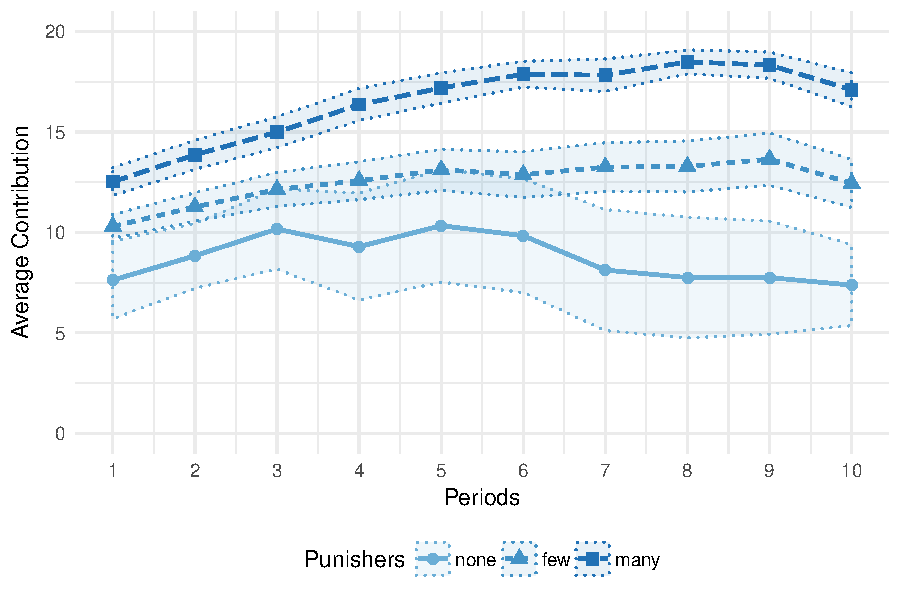
\includegraphics[width=.45\linewidth]{img/21_contrib}
     &&
    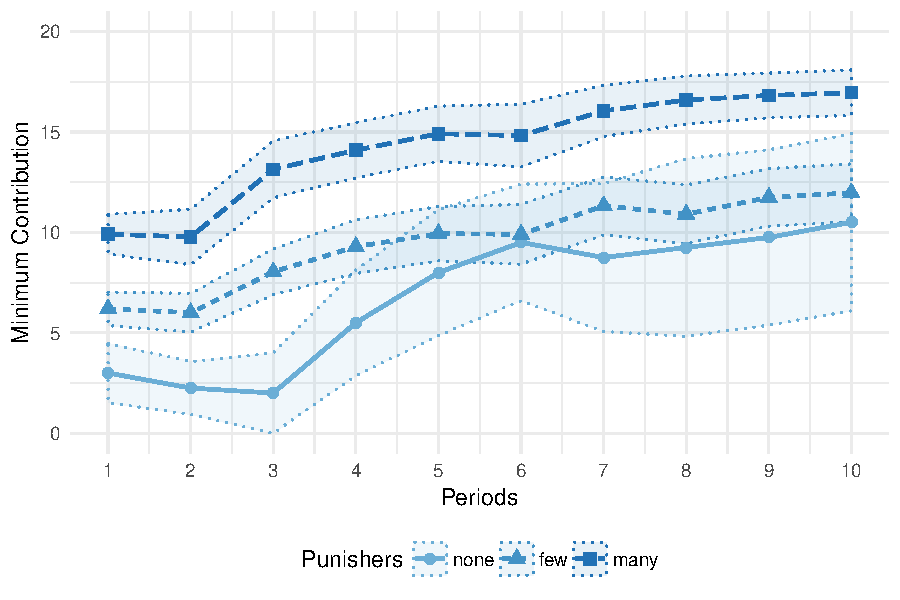
\includegraphics[width=.45\linewidth]{img/71_minimum}
        \\
    \hline
    \hline
    \multicolumn{3}{|c|}{Average Payoff $\bar{\pi}_i$}\\
    B&&E\\
    [.5em]
    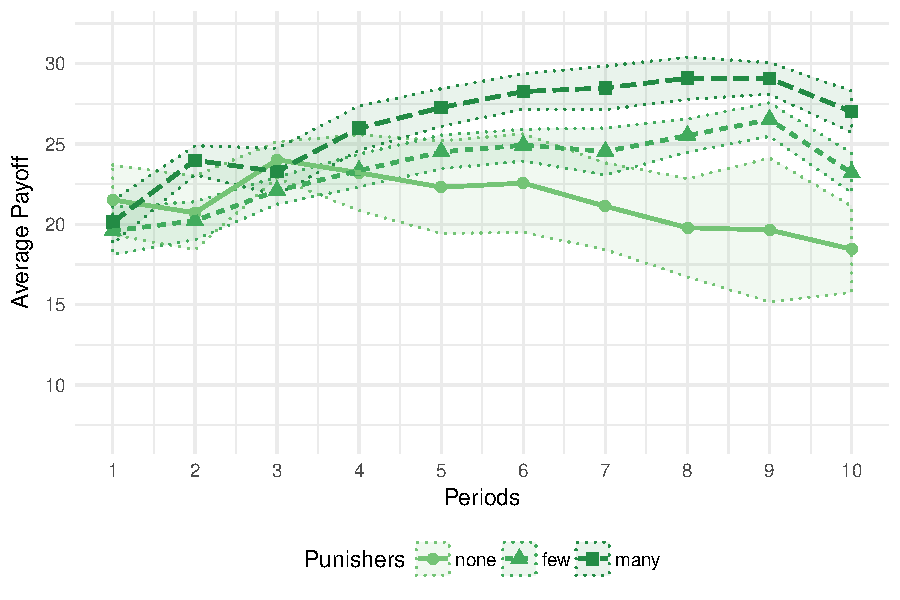
\includegraphics[width=.45\linewidth]{img/21_payoff}
     &&
    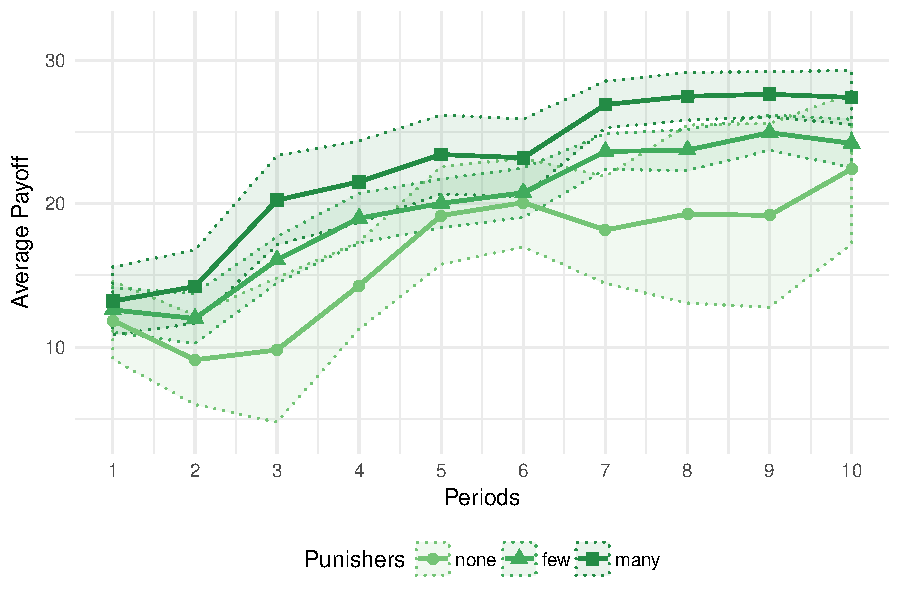
\includegraphics[width=.45\linewidth]{img/71_payoff}
        \\
    \hline
    \hline
    \multicolumn{3}{|c|}{Average Punishment $\bar{d}_{ij}$}\\
    C&&F\\
    [.5em]
    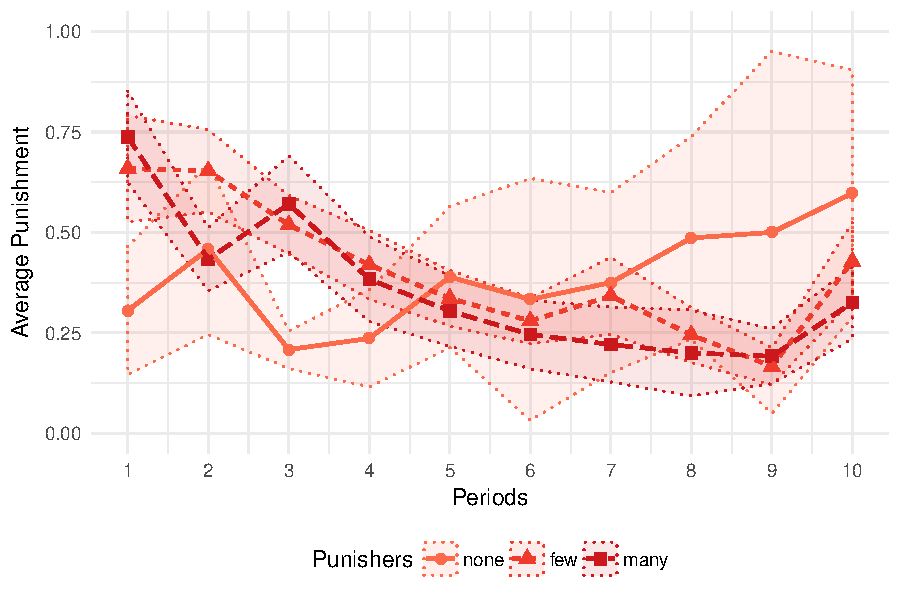
\includegraphics[width=.45\linewidth]{img/21_pun}
     &&
    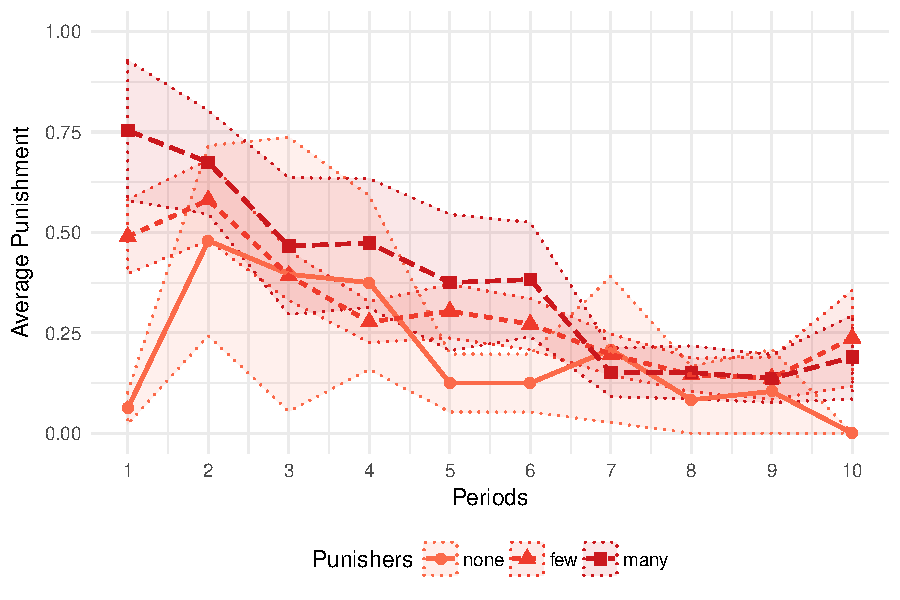
\includegraphics[width=.45\linewidth]{img/71_pun}
        \\
    \hline
  \end{tabular}
  \caption{Average Group Outcomes by Type Prevalence}
  \label{fig:groupout}
  \smallskip
  \parbox{\linewidth}{\footnotesize\textit{Note:} More than 65\% of subjects
    remain consistent across these two games in their punishment behavior.}
\end{figure}


\subsection{Payoff Comparison}


\end{refsection}

\begin{table}[htbp]
  \centering
  \caption{Mean Contribution $g_i$ in RP- and WP-game}
  \begin{tabular}[h]{rd{3}d{3}}
    \toprule
    & \mco{1}{$\mu_{g_i}$} & \mco{1}{$SE$}\\
    \midrule
    $RP$ & 10.798 & (0.457) \\
    $WP$ & 13.447 & (0.397) \\
    \midrule
    \mco{2}{t-test} & 0.000               \\
    \bottomrule
  \end{tabular}
  \label{tab: }
  \smallskip                          \\
  \parbox{\linewidth}{\footnotesize\textit{Note:}  }
\end{table}

\end{document}
end{document}




% linear
\begin{table}[htbp]
  \centering
  \caption{ }
\begin{tabular}{r*{4}{d{4}}}
\toprule
  & \mco{4}{Individually Assigned Punishment $d_{ij}$}\\
                      & \mco{1}{(1)}   & \mco{1}{(2)}   & \mco{1}{(3)}   & \mco{1}{(4)}    \\
\midrule
$g_i-g_j$             & 0.062^{***}    &                &                & 0.051^{***}     \\
                      & (0.005)        &                &                & (0.005)         \\
[.3em]
$d.RP\times(g_i-g_j)$ &                & 0.068^{***}    &                & 0.013^{*}       \\
                      &                & (0.007)        &                & (0.007)         \\
[.3em]
$d.WP\times(g_i-g_j)$ &                &                & 0.085^{***}    & 0.028^{***}     \\
                      &                &                & (0.007)        & (0.008)         \\
[.3em]
$d.RP$                &                &                &                & 0.166^{***}     \\
                      &                &                &                & (0.050)         \\
[.3em]
$d.WP$                &                &                &                & 0.100^{*}       \\
                      &                &                &                & (0.052)         \\
[.3em]
Intercept              & 0.443^{***}    & 0.624^{***}    & 0.539^{***}    & 0.461^{***}     \\
                      & (0.009)        & (0.005)        & (0.024)        & (0.032)         \\
\midrule
Observations          & \mco{1}{6,840} & \mco{1}{6,840} & \mco{1}{6,840} & \mco{1}{20,520} \\
Adjusted \(R^{2}\)    & 0.215          & 0.222          & 0.251          & 0.212           \\
\bottomrule
\end{tabular}
 \label{tab:linear}
  \smallskip                                                                               \\
  \parbox{\linewidth}{\footnotesize\textit{Note:} Pseudo panel estimation with
    individual level fixed effects for 228 subjects. Cluster robust standard errors in
    parentheses.  P-values: 0.1 / 0.05 / 0.01 : * / ** / ***. (1) Only P-game, (2) Only RP-game,
    (3) only WP-game observations with 30 observations per subjects in each game. $g_i$ is individually constant within each
    game. Taking the difference $g_j$ and $g_i$ \emph{normalizes}
    observations of the P-, RP-, and WP-game creating a single kink
    for all three games.}
\end{table}

% linear
\begin{table}[htbp]
  \centering
  \caption{ }
\begin{tabular}{r*{4}{d{4}}}
\toprule
  & \mco{4}{Individually Assigned Punishment $d_{ij}$}\\
                      & \mco{1}{(1)}   & \mco{1}{(2)}   & \mco{1}{(3)}   & \mco{1}{(4)}    \\
\midrule
$g_i-g_j$             & 0.062^{***}    &                &                & 0.051^{***}     \\
                      & (0.005)        &                &                & (0.005)         \\
[.3em]
$d.RP\times(g_i-g_j)$ &                & 0.068^{***}    &                & 0.013^{*}       \\
                      &                & (0.007)        &                & (0.007)         \\
[.3em]
$d.WP\times(g_i-g_j)$ &                &                & 0.085^{***}    & 0.028^{***}     \\
                      &                &                & (0.007)        & (0.008)         \\
[.3em]
$d.RP$                &                &                &                & 0.166^{***}     \\
                      &                &                &                & (0.050)         \\
[.3em]
$d.WP$                &                &                &                & 0.100^{*}       \\
                      &                &                &                & (0.052)         \\
[.3em]
Intercept              & 0.443^{***}    & 0.624^{***}    & 0.539^{***}    & 0.461^{***}     \\
                      & (0.009)        & (0.005)        & (0.024)        & (0.032)         \\
\midrule
Observations          & \mco{1}{6,840} & \mco{1}{6,840} & \mco{1}{6,840} & \mco{1}{20,520} \\
Adjusted \(R^{2}\)    & 0.215          & 0.222          & 0.251          & 0.212           \\
\bottomrule
\end{tabular}
 \label{tab:linear}
  \smallskip                                                                               \\
  \parbox{\linewidth}{\footnotesize\textit{Note:} Pseudo panel estimation with
    individual level fixed effects for 228 subjects. Cluster robust standard errors in
    parentheses.  P-values: 0.1 / 0.05 / 0.01 : * / ** / ***. (1) Only P-game, (2) Only RP-game,
    (3) only WP-game observations with 30 observations per subjects in each game. $g_i$ is individually constant within each
    game. Taking the difference $g_j$ and $g_i$ \emph{normalizes}
    observations of the P-, RP-, and WP-game creating a single kink
    for all three games.}
\end{table}

% test _b[sdiffop] = _b[sdiffrp]
%( 1)  sdiffop - sdiffrp = 0
%      F(  1,   227) =    3.79
%           Prob > F =    0.0528

% test _b[sdiffrp] = _b[sdiffwp]
%( 1)  sdiffrp - sdiffwp = 0
%      F(  1,   227) =    4.09
%           Prob > F =    0.0443



% piecewise linear estimation
\begin{table}[htbp]
  \centering
  \caption{Piecewise linear estimation for punishment of subjects with lower and
  higher contributions than oneself}
\begin{tabular}{l*{4}{d{5}}}
\toprule
                              & \mco{1}{(1)}   & \mco{1}{(2)}   & \mco{1}{(3)}   & \mco{1}{(4)}    \\
\midrule
$\max(g_j - g_i;0)$           & 0.003          &                &                & -0.010^{**}     \\
                              & (0.005)        &                &                & (0.005)         \\
[.3em]
$\max(g_i - g_j;0)$           & 0.105^{***}    &                &                & 0.097^{***}     \\
                              & (0.008)        &                &                & (0.009)         \\
[.3em]
$d.RP\times\max(g_j - g_i;0)$ &                & -0.006         &                & 0.002           \\
                              &                & (0.007)        &                & (0.007)         \\
[.3em]
$d.RP\times\max(g_i - g_j;0)$ &                & 0.133^{***}    &                & 0.031^{**}      \\
                              &                & (0.012)        &                & (0.014)         \\
[.3em]
$d.WP\times\max(g_j - g_i;0)$ &                &                & -0.002         & 0.002           \\
                              &                &                & (0.008)        & (0.009)         \\
[.3em]
$d.WP\times\max(g_i - g_j;0)$ &                &                & 0.127^{***}    & 0.031^{**}      \\
                              &                &                & (0.011)        & (0.013)         \\
[.3em]
$d.RP$                        &                &                &                & 0.043           \\
                              &                &                &                & (0.048)         \\
[.3em]
$d.WP$                        &                &                &                & 0.038           \\
                              &                &                &                & (0.059)         \\
[.3em]
Intercept                     & 0.040          & 0.068          & 0.092          & 0.037           \\
                              & (0.047)        & (0.063)        & (0.072)        & (0.049)         \\
\midrule
Observations                  & \mco{1}{6,840} & \mco{1}{6,840} & \mco{1}{6,840} & \mco{1}{20,520} \\
Adjusted \(R^{2}\)            & 0.301          & 0.359          & 0.320          & 0.293           \\
\bottomrule
\end{tabular}
  \label{tab:piecewise}
  \smallskip                                                                                       \\
  \parbox{\linewidth}{\footnotesize\textit{Note:}  }
\end{table}


\begin{figure}[htbp]
  \centering
  \caption{Average punishment assigned for deviations from one's own contribution}
  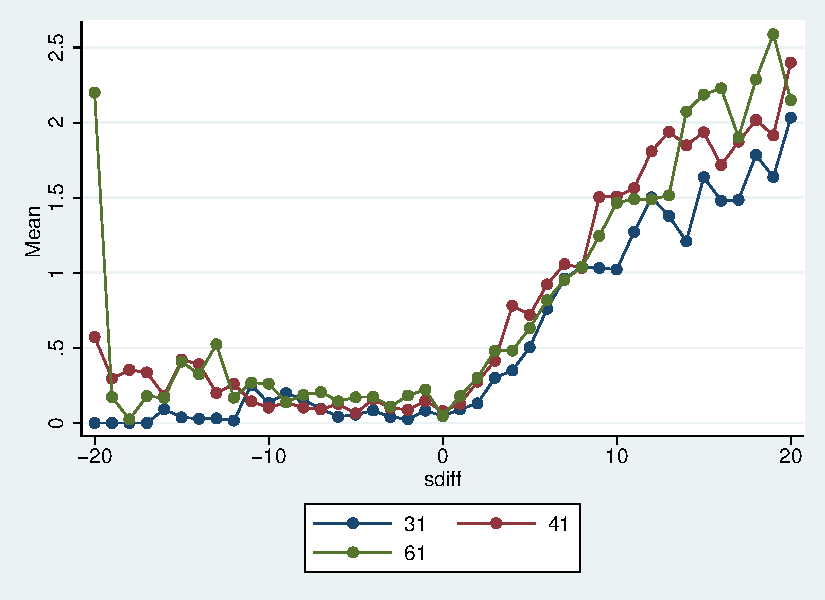
\includegraphics[width=.7\linewidth]{OUTPUT/lgraph_sdiff_PRPWP}
  \label{fig:sdiff}
  \smallskip\\
  \parbox{\linewidth}{\footnotesize\textbf{Note:} The x-axis shows the level
    deviation $g_i-g_j$from the punisher's own contribution level $g_i$ by the
    punished individual $g_j$. As shown in Albrecht and Traxler (2017)
    individuals predominately punish others with respect to their own
    contribution level, adapting punishment to whether subjects contributed more
    or equal $g_i-g_j \leq 0$ or less $g_i-g_j > 0$ than themselves.}
\end{figure}


\section{Design and Procedures}
The core of the experiment consists of a one-shot linear public good game with costly peer pu\-nish\-ment and the first period of a 10  period repeated public good game with costly punishment in a partners setting as found in \cite{Fehr2000}.
The punishment stage in the one-shot game and in the first period of the repeated game implement a strategy method on the punishment stage \citep{Kube2011}.
Exogenous variation in the contributions subjects faced in the strategy method implementation allows for consistent estimation of punishment behavior and isolation of retribution and deterrence motives across the two settings. 

\subsection{One-Shot}
The one-shot linear public good game with costly punishment is implemented in the spirit of \cite{Fehr2000,Fehr2002}. At the beginning of the game subjects are randomly assigned into groups of four. Each subject $i \in \{1..4\}$ is endowed with 20 tokens and has to decide how many tokens to contribute to the public good, $g_i$, and how many to keep for himself, $20-g_i$. Each token allocated to the public good yields a marginal per capita return of 0.4 MU. At the second stage of the game, each subject $i$ can assign punishment points to the other group members $j \neq i$, $d_{ij} \geq 0$. Assigning 1 punishment point costs 1 token for the punisher (1) and reduces the payoff of the punished subject by 3 tokens (2) \citep{Fehr2002,Herrmann2008}. The payoff function is therefore:
\begin{align}
    \pi_i = \underbrace{20 - g_i + 0.4\sum_{j=1}^4{g_j}}_\textrm{VCM}\underbrace{- 1\sum_{j\neq i}{d_{ij}}}_\textrm{(1)}\underbrace{- 3\sum_{j\neq i}{d_{ji}}}_\textrm{(2)} .
    \label{eq:pun}
\end{align}
Under the assumption of rational selfishness, the unique subgame-perfect Nash equilibrium is zero punishment and zero contributions to the public good.

We innovate on \cite{Fehr2000,Fehr2002} and the subsequent literature that used this design to study costly punishment in that we implement a novel variant of the strategy method at the punishment stage.\footnote{The procedure was first applied by \cite{Kube2011}. A similar approach -- called `Conditional Information Lottery (CIL)' -- is used in \cite{Bardsley2000}. However, the CIL was applied at the contribution rather than the punishment stage.\cite{Cheung2014} uses a strategy method on the punishment stage in a public good games but reduces the group size to 3 subjects and drastically truncates the range of contribution decisions.} In the first stage of the game, subjects make their contribution decision. In the second stage, subjects are confronted with a sequence of contribution triples of the other group members and have to decide on assigning punishment points to other subjects. The details of the procedure are as follows: each subject $i$ faces 11 screens, where each screen presents one contribution triple: $\{g^t_j , g^t_k , g^t_l \}$, with $t \in [1,11]$; the subindices denote the contributions of the other group members, $i \neq j \neq k \neq l$. One of the 11 triples is given by the actual, `real' contribution decisions made by the other group members. The remaining ten triples are hypothetical combinations of contributions, each being randomly drawn from a pre-defined set of combinations (see below). In addition, we also randomize the sequence at which individuals face these triples. For each triple, a subject has to decide how many punishment points (if any) to allocate to the other subjects.
% -----------

As the experiment aims at eliciting punishment behavior in a natural way it is important that subjects face contributions from the entire strategy space  while at the same time avoiding boredom and overstraining people with too many situations.
We therefore partition the strategy space into three intervals: \textit{low (L)}, \textit{intermediate (M)}, and \textit{high (H)} contributions with $g^L \in \{0,...,4\}$, $g^M \in \{5,...,15\}$, $g^H \in \{16,...,20\}$.
Based on these partitions, we considered 10 combinations of low, intermediate and high contributions:\\ \smallskip
 \begin{table}[ht!]
    \centering
    \begin{tabular}{|ccccc|}
        \multicolumn{5}{c}{\textbf{Hypothetical:}}\\
        \hline
        $\{g^L,g^L,g^L\}$& $\{g^L,g^L,g^M\}$& $\{g^L,g^L,g^H\}$& $\{g^L,g^M,g^M\}$&$\{g^L,g^M,g^H\}$\\
        $\{g^L,g^H,g^H\}$&  $\{g^M,g^M,g^M\}$& $\{g^M,g^M,g^H\}$&$\{g^M,g^H,g^H\}$&$\{g^H,g^H,g^H\}$\\
        \hline
        \multicolumn{5}{c}{}\\
        \multicolumn{5}{c}{\textbf{+ Real: }$\mathbf{\{ g_j,g_k,g_l\}}$}\\
    \end{tabular}
    \caption{Composition of Contribution Triplets}
    \label{tab:triplet}
\end{table}
%
Within each of the 10 hypothetical contribution combinations, we randomly draw from a set of 8 different triples (the triples are reported in the Online Appendix~A).
A subject could then face, for instance, $\{0,2,3\}$ for the combination $\{g^L,g^L,g^L\}$ and $\{1,2,10\}$ for $\{g^L,g^L,g^M\}$, etc.
A different subject might face $\{1,3,3\}$ for the former and $\{0,2,14\}$ for the later.\footnote{If, by chance, the triple $\{0,2,14\}$ would correspond to the real combination of contributions, the subject would not face this triple.
Instead a different triple from the pre-defined set of contribution triples for $\{g^L,g^L,g^M\}$ would be randomly drawn.}

All subjects know that 10 out of the 11 contribution triples are hypothetical.
It is also common knowledge that only the punishment decisions for the real contribution triple is payoff relevant. However, subjects neither know which one is the `real' triple, nor do they know the procedure to generate the hypothetical triples. Only at the end of the experiment the `real' contribution triple and punishment choices are revealed. Following this protocol, we observe $3 \times 11$ punishment decisions for each subject. As discussed below, our analysis will explore only the choices made for the 30 hypothetical contributions.
%As is depicted in table \ref{tab:triplet}.



\subsection{Repeated}
The secondary game is 10 period repeated linear public good game with costly punishment in a partners setting in the tradition \cite{Fehr2000}. The game uses the same payoff function as the one-shot game. In the beginning of the  repeated game subjects are randomly assigned to groups of 4 individuals and remained in these groups for the entire 10 periods. In the punishment stage of the first period  subjects, like in the one-shot game, are presented with 11 scenarios consisting of hypothetical and real contribution triples. Once all subjects have completed the 11 triples of the first round, subjects are presented with the payoff obtained in period 1. After this subjects continue to play the public good game while remaining together with the same subjects in one group. In the subsequent period 2 to 10, however, subject do not face hypothetical triples but are only presented with the real contributions of the other subjects.

We made clear to subjects that the group composition in all 10 periods would remain constant and that they would interact repeatedly. This was so that the prospect of future payoffs being dependent on other players' behavior was especially salient. The deterrence aspect of punishment should be as clear as possible to subjects without actually mentioning potential strategic considerations in the instructions.



\subsection{Implementation}
%
%
We implemented the described setup for 452 subjects from the university of Bonn in Germany, 156 subjects from Waseda University in Tokyo -- Japan, and 140 subjects from Florida State University in Tallahassee -- Florida, between the summer of 2013 and spring of 2016.
The experiments were conducted in June 2013 in Bonn EconLab using the experimental software \textit{zTree} \citep{Fischbacher2007}.
Subjects were randomly recruited online using Orsee in Germany and Florida \citep{Greiner2004}.
Waseda university in Japan used the online announcement platform of the student's intranet to recruite student for the experiments.
Experimental materials were translated from the original German to both language using back and forth translations ensuring that the materials matched as closely as possible.
A native speaker of the respective language (English, Japanese) translated the instructions from their original German.
A German native speaker then back-translated into German.
This process was repeated to fine-tune translations to be as close as possible to the original without sounding out of place for the participants. 

To ensure that the experiments were conducted in an identical fashion one of the authors was present at all three locations supervising the local staff and controlling the zTree software.
However, to avoid potential experimenter effects only the local staff interacted with the experimental subjects.
In all three locations standard experimental procedures were followed. After subjects were randomly seated in the lab, they received a printed game description for the first game which was read out aloud to them\footnote{In Bonn and at FSU the descriptions were read aloud by local staff. At the Waseda lab the instructions were read to the subjects by a naturally sounding text-to-speech software as is common practice at Waseda. Though this deviates from the human read instructions in the other two locations, this approach was preferred over making changes to the usual practice at the Waseda lab.}. Before they could proceed to the game interface a number of control questions had to be answered to verify their understanding of the first game. The one-shot and the repeated interaction game were preceded by a one-shot VCM game with a strategy method known from \cite{Fischbacher2001}. You find a the game as part of the instructions. We do not consider results from the VCM here. After the first game had been completed by all, subjects received another set of instructions that was read out aloud to them and had to answer an additional set of control questions. Results and payoffs from the VCM game and the one-shot game were only revealed after the final game had finished.
To prevent strategic spillovers between games, subjects were only made aware of the following game after the previous one was completed by all subjects.
Subjects received and were read aloud the instructions to the repeated interaction game and had to answer an additional set of control questions. Results and payoffs from the repeated interaction game were revealed after each period.

Subjects took on average 100 minutes to complete all three games and the concluding questionnaire. Payoffs in all three locations were of similar magnitude. See table \ref{aptab:payoff} for a listing of the location specific average payoffs.

%Herrmann text:
%A second and very important instrument to minimize experimenter effects is to have written
%instructions that are the same everywhere, except for being written in the respective language. To ensure maximal comparability of instructions we first wrote them in German and English and then a native speaker of the respective language translated the instructions into the respec- tive language. Another native speaker translated them back into English. We fine-tuned the translations until we could be sure that the rules of the experiment were explained as similarly as possible. All participants also had to solve the same set of control questions that ensured that subjects understood the rules of the experiment and payoff calculations (see Section 1.4 for a sample copy of the instructions and the control questions, and Section 1.5 for the procedures used)


